In this chapter, we will at first introduce the basic notions of IP multicast and IP mobility management protocol. We then present some background on multicast support in mobile environments, as well as its associated problems. In the scope of this thesis, we focus on the network-based mobility management protocol i.e., PMIPv6. Thus, we will sketch the existing proposals for multicast mobility support in PMIPv6 mainly from the IETF point of view regarding their advantages and limitations. Also, the multicast mobility in DMM will be discussed. 

\section{IP Multicast}
As Internet is widely deployed and spread across a large area, it carries a variety of common information resources and services. In a sharing world, group communication service, which refers to the ability to send data to several receivers at the same time, is naturally becoming more and more important especially in some areas such as multimedia distribution, gaming, and financial services, etc. In this context, IP multicast offers an effective and scalable mechanism to support group communication applications. 

Unlike the traditional communication model where data is sent from a source to a destination (called unicast or one-to-one model) or to all the nodes in a specific scope (broadcast), multicast allows transmitting data to a set of users that are interested in receiving data destined to a specific group, referred to as a multicast group. Internet Protocol (IP) multicast (or IP multicast) was first proposed by Steve Deering in the late 1980s \cite{Deering_88}, and was then standardized by IETF in RFC 1112 \cite{RFC1112}. IP multicast describes how nodes can send and receive multicast packets across IP networks. The first multicast session was executed to transfer the audio multicast over the Internet via the Multicast Backbone (MBone) in 1992 \cite{developing_ip_multicast,Mbone}.   

In multicast, the sender only needs to send a single copy of data to reach all the group members, rather than sending a separate copy to each receiver. The intermediate routers then duplicate data packets until they reach the receivers. As a result, the multicast brings some advantages compared to the unicast and the broadcast mode such as efficient delivery to multiple destinations (e.g., reducing server load and eliminating traffic redundancy), thus improving overall resource utilization \cite{developing_ip_multicast}. 

A multicast source can send the multicast data to the group at any time, without the need for prior registration/scheduling and joining the group. If a source desires to send data packets to the multicast group, it uses the group address as the destination address in its data packets. Moreover, the source is usually unaware of any group membership details. Similarly, from receiver point of view, a host may join or leave a multicast group at any time without any restrictions on the location and the number of hosts in a group. Each multicast group is represented by an IP multicast address. The multicast address assignment is responsible by the Internet Assigned Number Authority (IANA)\footnote{http://www.iana.org}, as specified in \cite{iana_multicast_address}. 

After more than a decade of important researches and development efforts, IP multicast, in general, has been slowly deployed on the global Internet. The barrier of widespread deployment of multicast applications mainly comes from technical, administrative and business related issues as stated in \cite{alternative_multicast}. Therefore, several alternative techniques for multicasting have been proposed \cite{alternative_multicast}, in which each alternative can be suitable for a specific environment. For example, application-layer multicast (ALM) \cite{application_multicast} in which the multicasting functionality is implemented at the application layer instead of at the network layer as IP multicast does not require the change in the network infrastructure. Data packets are replicated at the end hosts, instead of the network routers as in IP multicast. ALM is suitable, for example, for the mobile ad hoc network (MANET) applications. Although ALM is much easier to deploy compared to IP multicast, IP multicast outperforms ALM (as well as other alternatives) in terms of robustness, security, performance, and scalability \cite{alternative_multicast}. The new business models \cite{ericsson_LTE}, a huge traffic demand (especially multimedia traffic), the revenue per data reducing phenomenon in the mobile operator networks, as well as the advantages of new multicast model (SSM) bring again the strong interest of IP multicast from both academy and industry. IP multicast is expected to play more important role in the future networks. As a result, this thesis focuses only on the case where multicast functionality is located at the network layer or IP multicast.  

Since IP multicast is based on the User Datagram Protocol (UDP) as a transport protocol, which only provides best-effort delivery guarantees, multicast packets are delivered without reliability or congestion control (at the transport layer). For applications that require a reliable data transfer, additional mechanisms must be provided by the application layer e.g., reliable multicast transport protocols.
\begin{figure}[h!] 
 \begin{center} 
 \includegraphics[width=0.60\textwidth]{./Part1/Chapter2/figures/c2_multicast_architecture.eps} 
    \caption[An example of multicast deployment architecture]{An example of multicast deployment architecture.}
     \label{fig:c2_multicast_architecture}
  \end{center} 
\end{figure}

\begin{figure}[h!] 
 \begin{center} 
 \includegraphics[width=0.85\textwidth]{./Part1/Chapter2/figures/c2_multicast_deployment.eps} 
    \caption[A multicast deployment scenario: from protocols point of view]{A multicast deployment scenario: from protocols point of view.}
     \label{fig:c2_multicast_deployment}
  \end{center} 
\end{figure}

In order to provide multicast service, two groups of protocol need to be deployed: multicast group membership protocols and multicast routing protocols. The multicast group membership protocols enable hosts to dynamically join/leave the group as well as make multicast routers (MR) aware of the interested receivers and manage their subscriptions. The multicast routing protocols enable a collection of MRs to build distribution trees to deliver the multicast traffic from sources to all the members of a multicast group.
The multicast group membership protocols, depending on IP version, are Internet Group Management Protocol (IGMP) \cite{IGMPv3} for IPv4 and Multicast Listener Discovery (MLD) \cite{MLDv2} for IPv6. 

Regarding the multicast routing protocols, each protocol uses its multicast routing algorithm to build the multicast delivery tree. There are many multicast routing protocols such as Distance Vector Multicast Routing Protocol (DVMRP) \cite{DVMRP}, Multicast Open Shortest Path First (MOSPF) \cite{MOSPF}, Core Based Tree (CBT) \cite{CBT,CBTv2}, Protocol Independent Multicast – Dense Mode (PIM-DM) \cite{PIM_DM}, and Protocol Independent Multicast – Sparse Mode (PIM-SM) \cite{PIM_SM}. 
In this thesis, the considered multicast routing protocols are PIM-SM and the enhanced version of PIM-SM for source specific (PIM-SSM \cite{PIM_SM}). To avoid deploying a full-stack MR inside a given network due to its implementation and operational costs, IGMP/MLD proxy \cite{MLD_proxy} which performs membership management, acts as a multicast Querier for its subnet and as a host for an upstream proxy/MR, is introduced. 

Fig.~\ref{fig:c2_multicast_architecture} and Fig.~\ref{fig:c2_multicast_deployment} show an example of a multicast deployment scenario from architecture and protocol point of view, respectively. As seen in Fig.~\ref{fig:c2_multicast_architecture}, multicast sources/listeners can be a mobile node or a fixed node. The multicast traffic is routed from the sources to the listeners via the intermediate MRs and/or MLD proxies. 

\subsection{IP Multicast Applications}
Taking advantages of multicast, various applications which can be classified into different groups following different criteria can be deployed. In terms of multicast model, the multicast applications can be placed into three main categories, as stated in \cite{multicast_applications,multimedia_multicast}:
\begin{itemize}
\item One-to-many (a single source sending to a set of receivers):  A typical example is scheduled audio/video distribution (including Internet Protocol Television (IPTV), mobile TV, lectures, presentations, etc.). Also, the multicast application can be used to push media like news headlines, weather updates, sport scores and financial services. Software update also falls into this category. 
\item Many-to-many (multiple sources sending to a set of receivers): Applications such as audio/video conferencing, distributed online games, and collaborative environments, in which some or all the participants become sources, are examples of the many-to-many model. 
\item Many-to-one (multiple sources sending to a receiver): Many-to-one applications include resource discovery (e.g., service location and device discovery), data collection (monitoring applications, video surveillance), and so on.  
\end{itemize}

Following the service function, these applications fall into such groups as Mobile TV (live and interactive TV), Personal Broadcasting Service (PBS), Live Video Distribution (conferences, seminars, etc.), Multimedia Content Distribution (Video On-Demand), General Content Distribution (Data on Demand, Online Gaming), and Machine-to-Machine Distribution (e.g., Software distribution and navigation system updates) \cite{multicast_3g_networks}. 
 
 \subsection{Multicast Model}
At the time IP multicast was introduced, a \textit{host group} model supported both one-to-many and many-to-many group communication (referred as Any-Source Multicast, or ASM). However, this model is also one of the main barriers for the widely multicast deployment. It is due to the fact that there are several deployment issues of the ASM model such as multicast address allocation and management, lack of access control (leading to the denial of service attacks), scalability and service provisioning \cite{overview_SSM,SSM}.   

To promote the deployment of multicast, a new service model, the so-called Source-Specific Multicast (SSM), is introduced. The great advantage of SSM is the simplicity. SSM model also overcomes the limitation of ASM and is suitable for one-to-many applications. 
A range of multicast addresses (FF3x::/32 for IPv6) is reserved for SSM. In more details, SSM simplifies the multicast related mechanism by eliminating the need of the Rendezvous-Point Tree (RPT), RP, and Multicast Source Discovery Protocol (MSDP)\footnote{ The control plane for source discovery is now under the responsibility of receivers}. To cope with SSM model, the group management protocol is required to support source filtering as described in \cite{MLD_SSM}. Also, PIM-SSM \cite{PIM_SM}, as an extension of PIM-SM, is specified to handle a source-specific model.

\subsection{Group Management Protocols}
Multicast group membership protocols consist of two parts. The first part, namely multicast listener one, is used by hosts/routers to announce their interest in receiving traffic destined to a specified group with their neighboring MRs. 
The second part, multicast router one, is performed by the MRs to discover the presence of the interested hosts of a given group and to manage their subscriptions for each of their directly attached link. IETF defines two multicast group membership protocols, i.e., IGMP \cite{RFC1112, IGMPv2, IGMPv3} for IPv4 and MLD \cite{MLDv1,MLDv2} for IPv6. The current version of IGMP (IGMPv3 \cite{IGMPv3}) and MLD (MLDv2 \cite{MLDv2}) share the same functionality. In this thesis, only MLDv2 is considered since we focus on the IPv6 network. The interaction between the two parts is done by using MLD messages. 

From a multicast listener point of view, when the upper-layer protocols or application programs ask the IP layer to enable the reception of multicast traffic from a specific multicast address, a node will send an MLD Report message to its MR to join this group. The MR then joins the multicast group (if necessary) and forwards the multicast packets to the subscribed nodes. The MLD Report is also used to reply to the general queries which are periodically sent by the MR to learn about the multicast subscription information from an attached link. In addition, if the listening state of a node changes, the node will immediately report this change via a State Change Report message.

From an MR point of view, the MR uses MLD to learn, for each of its directly attached links, which multicast addresses and which sources have listeners interested on that link (to support SSM). Thus, the router only needs to know whether there is at least one group member per network interface which is interested in receiving the multicast traffic of a multicast group, or not. However, the router can maintain the detailed subscription information regarding the multicast addresses, their corresponding subscribed hosts, and the associated network interface by means of the explicit tracking function \cite{explicit_tracking}. Enabling the explicit tracking function can help reduce the multicast-related issues in a wireless environment such as signaling overhead and leave latency. 

The basic operations of MLD are briefly described as follows:
\begin{itemize}
\item One MR in a subnet, the so-called Querier \cite{MLDv2}, periodically sends MLD General Query messages onto the link to build and update the multicast membership state of all multicast routes on this link. 
\item Nodes respond to these queries by sending a Current State Report message indicating their group memberships to all MLDv2 routers on the link. Whenever their listening state changes, they report these changes to the routers via a State Change Report message. 
\item All routers, upon the reception of the Report messages, update the memberships state on the link. If the Querier receives an MLD State Change Report indicating that the node desires to stop listening to a particular group, the Querier will make a query for the presence of other listeners subscribed to this group using a Multicast Address Specific Query, before deciding to stop forwarding multicast traffic for this group. Similarly, the Multicast Address and Source Specific Query is used to learn the membership state of a specified multicast address with specified source address. 
\item If a router does not receive a Report message for a particular group for a period of time, it will assume that there are no more members of the group on the link and can stop forwarding the multicast packets for this group. 
\end{itemize}

\subsection{Multicast Routing Protocols}
IP multicast does not require a source sending to a given group to know about the receivers of the group, instead it is based on the multicast delivery trees to deliver the multicast packets. Multicast routing protocols are responsible for building the multicast delivery trees and forwarding the multicast packets along the trees to the appropriate receivers. Various multicast routing protocols, according to the type of the multicast tree they build, can be grouped into two categories: a source-based tree and a share tree. 

The source-based tree (or shortest-path tree) protocols are based on the shortest path towards the source to build a tree to minimize the path cost from the source to each receiver. Thus, such a separate delivery tree is built for each multicast source of a given group. In this case, the multicast packets will be delivered along a shortest-path tree from the source to the members of multicast group in order to meet the objective of a low-delay multicasting \cite{Deering_88}. Protocols such as DVMRP, MOSPF, PIM-SSM and PIM-DM use this kind of multicast delivery tree. 

For example, DVMRP is the first multicast routing protocol proposed by S. Deering \cite{Deering_88}. DVMRP is a flood-and-prune protocol in a sense that the source floods the multicast packets to the entire domain and the routers which do not have multicast listener for this group send a prune message to stop forwarding packet to them. In more details, the packets that do not arrive at a router on the appropriate interface (the interface from which the router could forward a unicast packet to the source following the shortest path) are ignored. Otherwise, they will be forwarded to all, except the incoming interface. Based on IGMP protocol, the leaf routers which do not have multicast listener for this group prune back to the spanning tree. However, the multicast packets need to be re-flooded to detect the new listeners. As a result, the prune messages need to be sent periodically to remove the unnecessary links along the shortest path tree towards the source. All together, it leads to the scalability issue.  

There is another type of algorithm, the so-called Shared Tree (or Core-based Tree) where a single tree is shared by all the sources of the same multicast group. In other words, the multicast traffic for each group is sent and received over the same delivery tree, regardless of the source. It is achieved by introducing a core router, the so-called Rendezvous Point (RP) which is a pre-defined router. The MR may statically store the address of RP or discover the address during the bootstrap phase \cite{PIM_SM}. When a source transmits a packet to a multicast group, the packet is first sent to the RP which then forwards the packet along the reverse shortest path tree (towards the RP) to reach all the listeners. Moreover, each edge router which desires to receive the multicast traffic has to join the tree by sending an explicit \textit{Join} message towards the RP. Based on that, the multicast delivery tree is built. Comparing to the previous algorithm, CBT is better regarding network bandwidth since it does not require the multicast packets to be periodically forwarded to all MRs in the internetwork. Protocols such as CBT and PIM-SM use the core-based tree. 

Additionally, the flooding mechanism is suitable for the case where the members of the multicast group are densely distributed across the network. These protocols using it as a distribution mechanism are called dense-mode protocols. On the contrary, in the widely distributed multicast environments where the group members are spread sparsely across the network, the flooding mechanism may cause a waste of bandwidth and performance issues. As a result, CBT with the explicit join mechanism is more suitable. The corresponding routing protocols are called the spare-mode ones. 

\subsubsection{Protocol Independent Multicast-Spare Mode/Source-Specific Mode}

The name of Protocol Independent Multicast (PIM) derives from the fact that PIM does not have its own unicast routing protocol, instead it relies on the existing unicast routing protocols to build a separate multicast forwarding table. PIM-Spare Mode (PIM-SM), a spare-mode protocol, is the most widely used multicast routing protocol. PIM-SM is a dual-stack protocol for both IPv4 and IPv6. However, in the scope of this thesis, we focus on IPv6 part of this protocol which uses both the source-based and the shared-tree to deliver the multicast traffic. 

In PIM-SM, a RP plays the role of a core of the multicast delivery tree in a sense that the source sends the multicast packet to the RP. When a listener wishes to receive multicast traffic from a group, it sends an MLD Report to its default MR (designated router or DR) which then joins the multicast delivery tree on behalf of the listener. As a result, the existence of the sources and the listeners are independent of each other. The detailed operation of PIM-SM is described as follows.

The PIM-SM operations consist of three phases as described in Fig.~\ref{c2_pim_operation}. In the phase one (see Fig.~\ref{fig:c2_pim_p1}), a multicast listener expresses its interest in receiving multicast traffic  destined for a given group by sending an MLD Report to its DR. The DR then sends a PIM Join message towards the RP for that group. Since the multicast traffic can arrive from any sources, the Join message is denoted as (*, G) Join. The MRs on the path towards the RP of the (*, G) Join establish the multicast tree state for group G. Therefore, a multicast delivery tree with the root at the RP is constructed for group G, called RP Tree (RPT). Since the RPT is shared by all the sources, it is considered as a shared tree. From a multicast source point of view, the source can start sending data packets destined for a group at anytime. The source's DR, upon receiving the multicast packets, unicast-encapsulates them and sends them directly to the RP (as known as the registering process). The RP, on the reception of the encapsulated packets, decapsulates them and forwards them natively following the multicast forwarding state onto the shared tree. The multicast packets are then replicated by the intermediate routers and reach the listeners. The encapsulation packets are called the PIM Register packets. 
\begin{figure}[h!]
\centering
\subfloat[]{\includegraphics[width=0.47\textwidth]{./Part1/Chapter2/figures/pim_p1.eps} \label{fig:c2_pim_p1}}\,
\subfloat[]{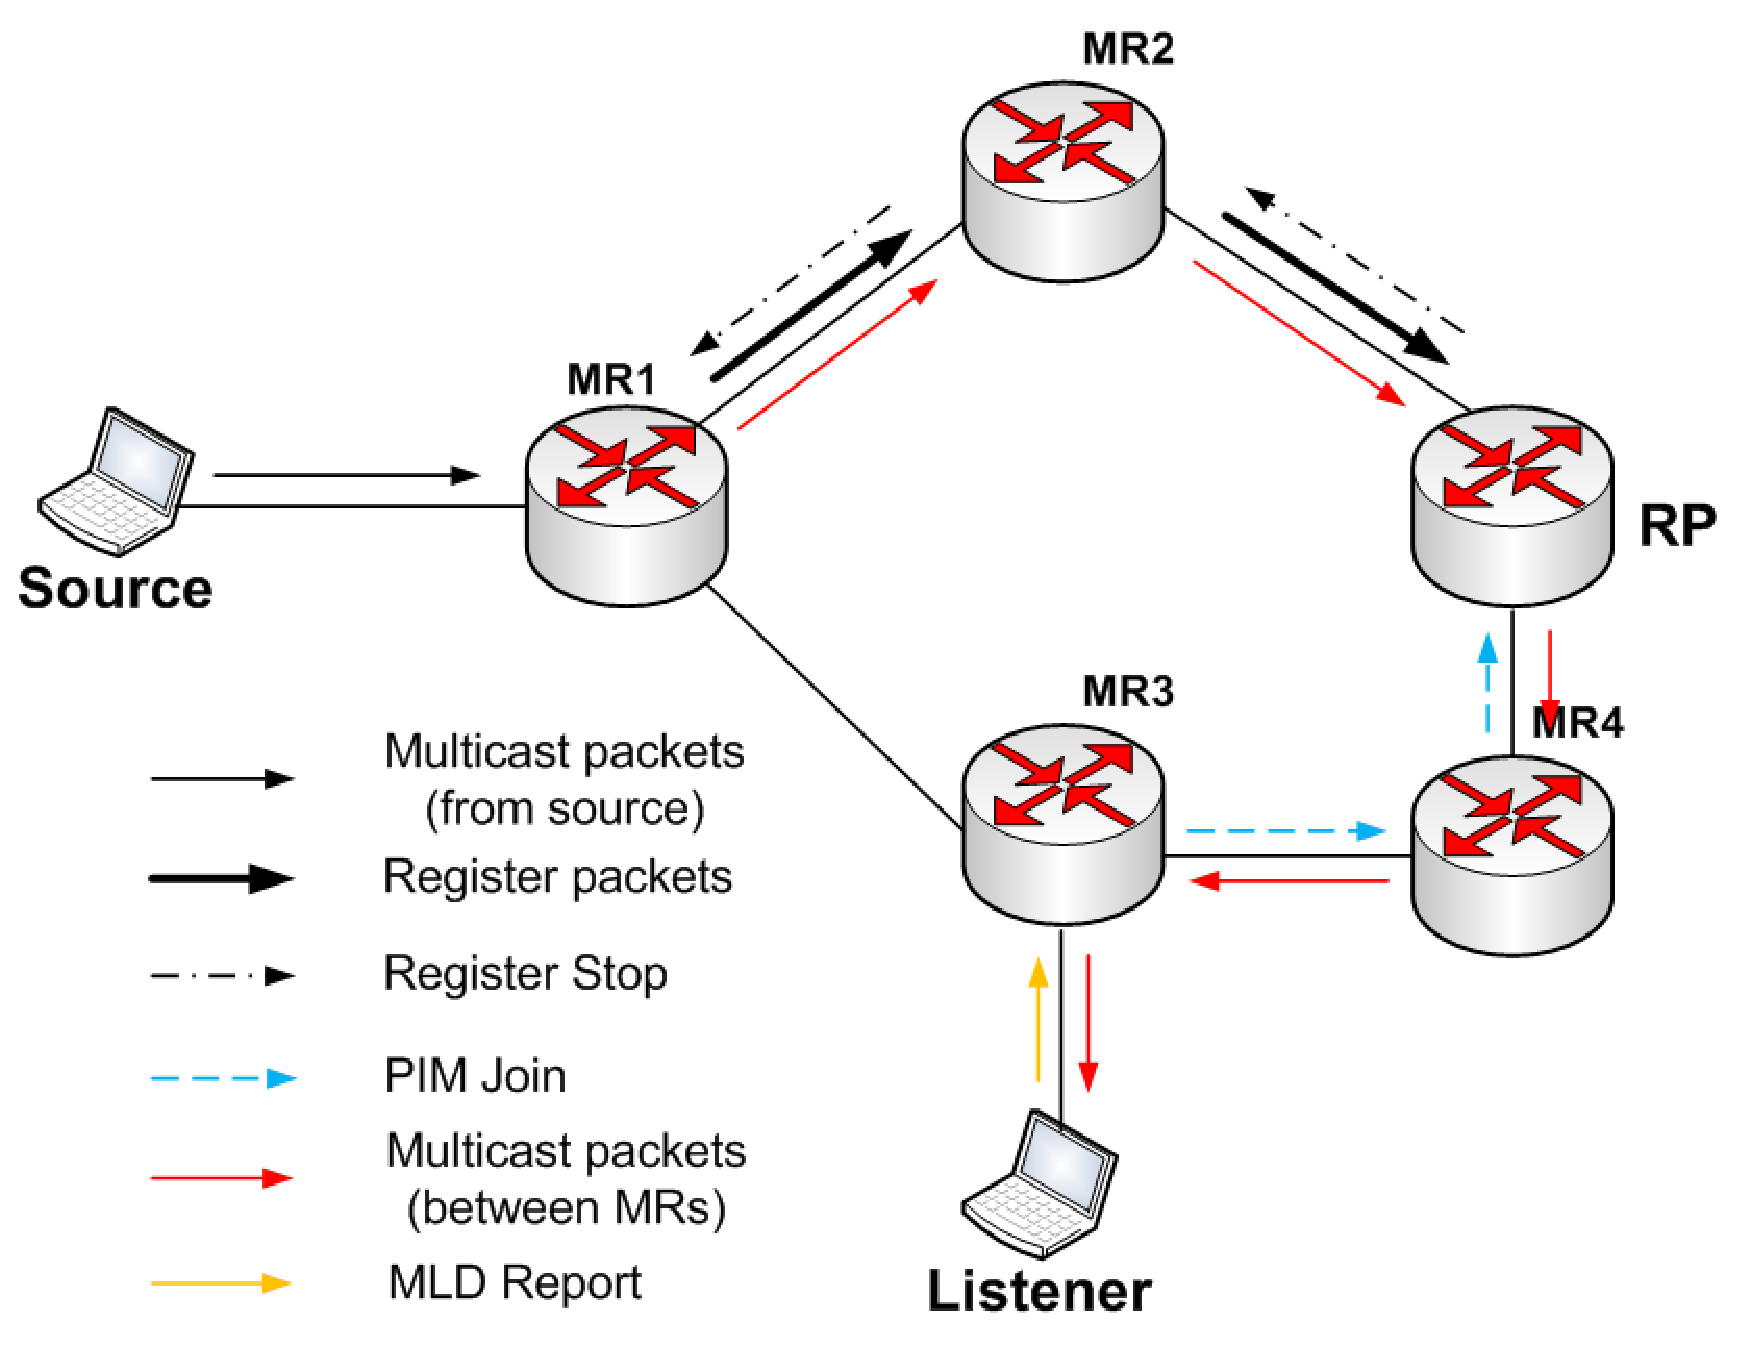
\includegraphics[width=0.47\textwidth]{./Part1/Chapter2/figures/pim_p2.eps}\label{fig:c2_pim_p2}}\,
\subfloat[]{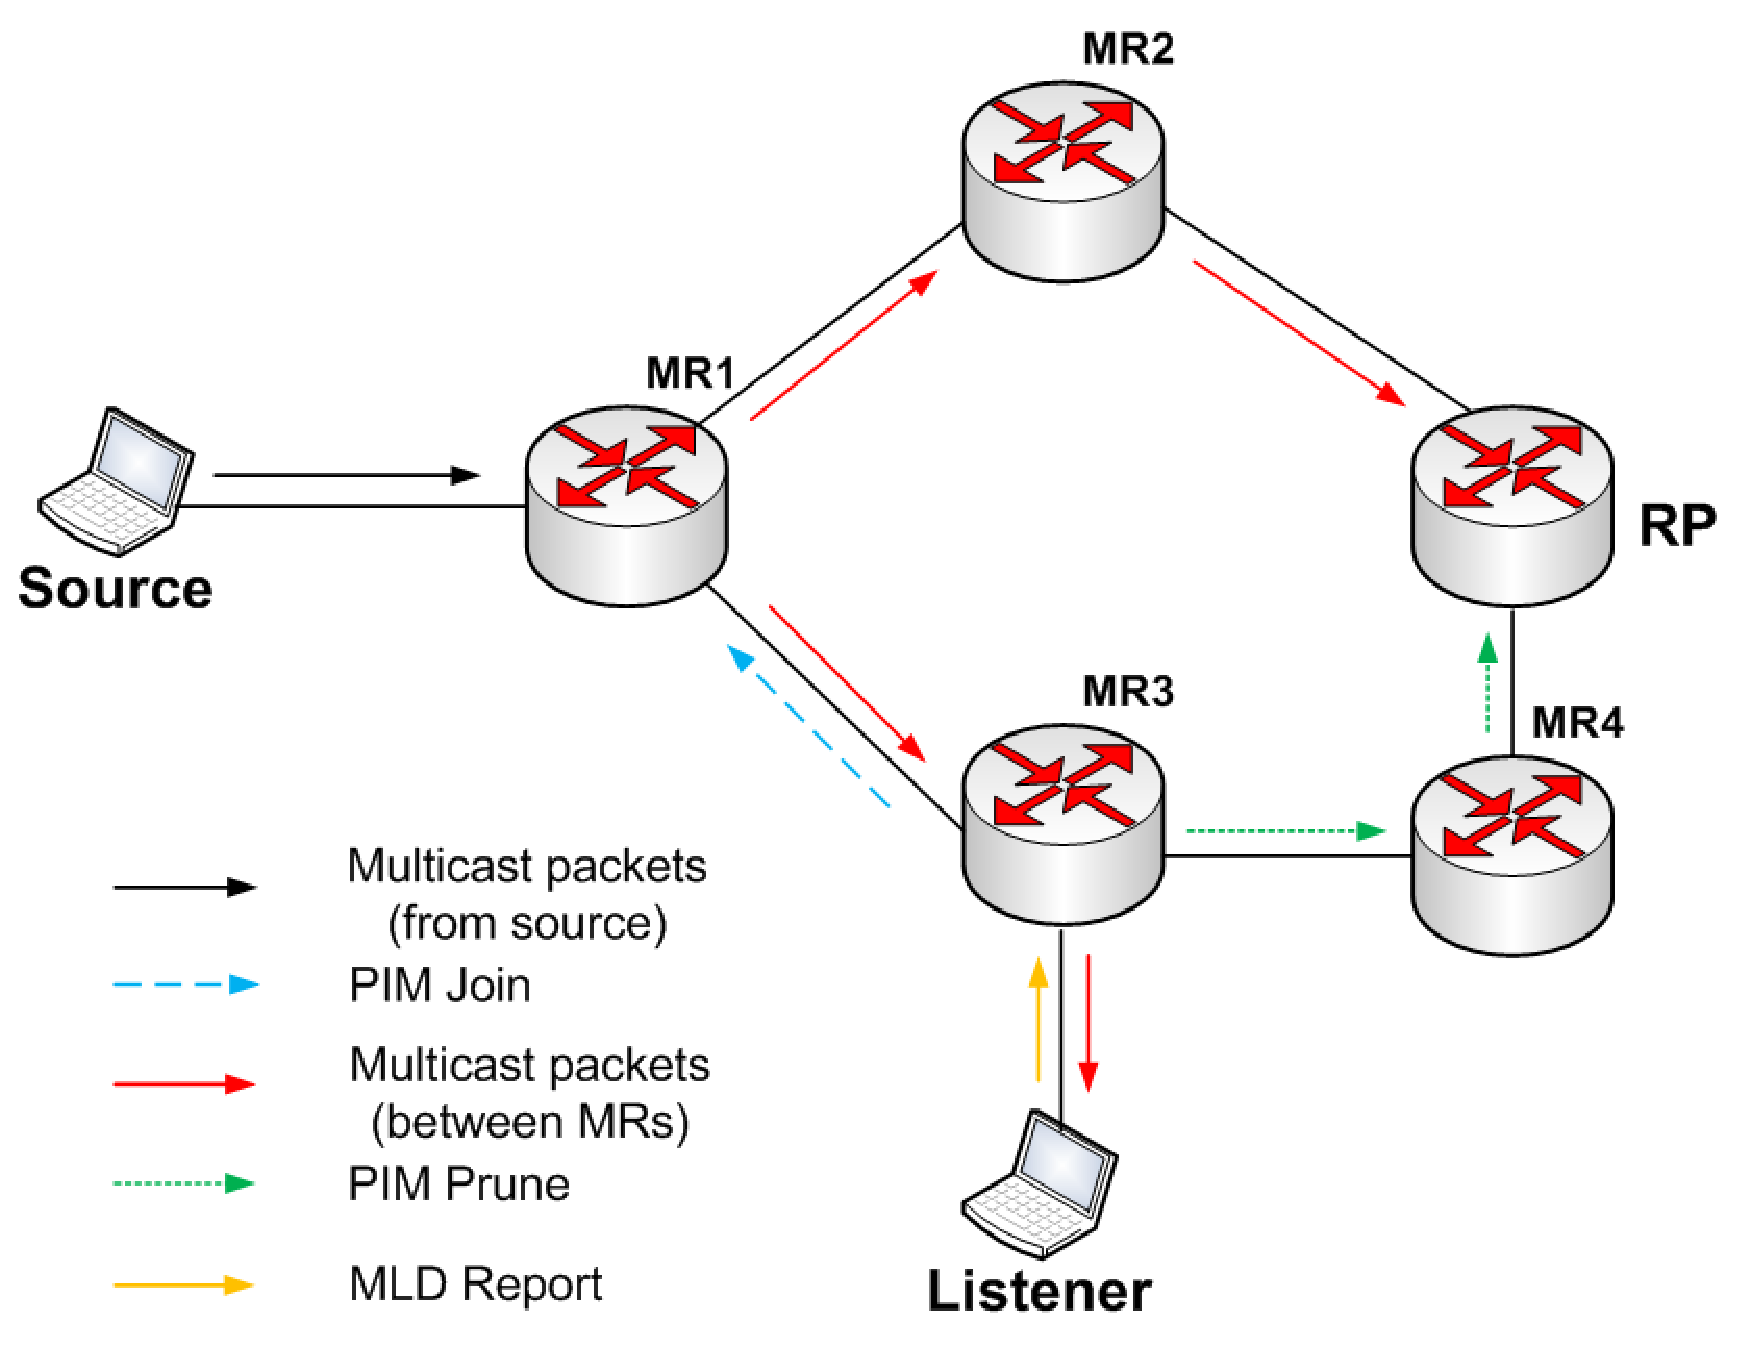
\includegraphics[width=0.47\textwidth]{./Part1/Chapter2/figures/pim_p3.eps}\label{fig:c2_pim_p3}}
\caption[The operations of PIM-SM]{PIM-SM operations: (a) phase 1, (b) phase 2, (c) phase 3.}
\label{c2_pim_operation}
\end{figure}

In the phase two (see Fig.~\ref{fig:c2_pim_p2}), after receiving the PIM Register packets from a source S, the RP may decide to switch to a native multicast forwarding by sending a (S, G) Join towards the source S. Similarly, the (S, G) multicast tree, which is the shortest-path tree towards the source S, will be established. In the meantime, the data packet will continue being encapsulated to the RP. As soon as the multicast packets arrive natively at the RP, the RP sends a Register-Stop message to inform the source's DR to stop encapsulating the packets. At the end of this phase, the traffic will be routed natively from source S to the RP, and then along the shared tree to the listeners.      

Fig.~\ref{fig:c2_pim_p3} illustrates the PIM operations in the phase three. As the traffic passes through the RP, it is usually not an optimal path from the source to the listener. Thus, the listener's DR may send a (S, G) Join towards the source to switch to the shortest path tree. Similarly, after receiving the multicast packets from the source, the listener's DR sends a Prune message to the RP (known as  (S, G, rpt) Prune) to prune the unnecessary routes. At the end of this phase, the multicast traffic is routed following a shortest-path tree from the source S to the listener. 

The SSM model can be enabled at a PIM-SM router by using a subset of the PIM-SM protocol mechanisms. In more details, from an MR point of view, only (S, G) Join/Prune messages are generated by the router, and no (*, G) and (*, G, rpt) Join/Prune messages are generated. The packets related to (*, G) or (S, G, rpt) state should be ignored. PIM-SSM is backward compatible with PIM-SM, that means the router can only implement a subset of PIM-SM for SSM support. 
 
\subsection{IGMP/MLD Proxy}
The operators, in some cases, may not desire to deploy the multicast routing function on the routers inside a given network due to the hardware, the implementation and operational cost of an MR. In this case, IGMP/MLD proxy (is referred as MLD proxy, from now on) \cite{MLD_proxy}, as a lightweight protocol compared to the complicated multicast routing protocols such as PIM and DVMRP, can be used to simplify the design and implementation of the router. It should be noted that MLD proxy only works in a single tree topology as can be seen in Fig.~\ref{fig:c2_multicast_architecture}. This proxy performs the router part of MLD protocol on its subnet and the host part on its upstream interface. In other words, the MLD proxy function allows an intermediate node to appear as an MR to the downstream hosts and as a host to the upstream MRs. The MLD proxy device maintains a database as a multicast membership. The MLD proxy will forward the multicast packets arriving from an upstream interface to all the downstream interfaces that have the subscription information of this group. Also, if a packet arrives at the proxy from a downstream interface, it will be forwarded to the upstream interface and to all the downstream interfaces that have the subscription information of this group except the incoming one. 

\section{IP Mobility Management}\label{c1:IP_Mobility}

Nowadays, the mobile data services have become an essential part of many consumers' lives \cite{cisco_forecast,data_services}. 
So far, the users have been using their mobile devices (e.g., smartphones and tablets) not only for personal life (e.g., making voice/video calls, sending email, watching video/TV, playing online games, and so on) but also for work (general and job-specific work applications such as multimedia conferencing, and distance learning, etc.) on a regular basic \cite{cisco_service,morgan_stanley, mobile_2010}. As a result, the mobile data traffic has been almost doubled each year during the last few years \cite{ericsson}. This trend is expected to continue in the upcoming years, especially with the deployment of 4G networks. The widely usage of mobile data services has been driven by the variety of different reasons such as: the increasing number of mobile devices which become more and more powerful and intelligent, the enhancement of wireless access technology in terms of coverage, speed and quality, as well as the explosion of mobile applications \cite{ericsson}. The mobility of the devices puts a new requirement on the mobile operators to provide connectivity anywhere and at anytime. Moreover, providing consistent and seamless services is required for satisfying user's expectations and fulfilling even highly application requirements in terms of service disruption on the move \cite{seamless}. 

In all-IP mobile networks, IP mobility is a crucial concept to meet the demand of ubiquitous Internet connectivity as well as new service requirements such as seamless handover across heterogeneous networks, consistent quality of experience and stringent delay constraints. IP mobility can be handled at different layers of protocol stack ranging from the link layer to the application layer \cite{RFC6301, survey_mobility_management, mobility_handoff_management}. The link layer mobility management protocols use the underlink information for mobility-related procedures when the MN roams among different physical points of attachment while keeping its layer 3 attachment (preservation of the IP address). The transport layer mobility management protocols  \cite{transport_layer_snoeren, transport_layer_Atiquzzaman} provide an end-to-end mobility support without requiring to change the network layer infrastructure. Regarding the mobility protocols at the application layer, the most well-known protocol, Session Initiation Protocol (SIP) \cite{SIP_mobility,SIP_application_layer}, provides an end-to-end mobility management framework, which does not depend upon the network entities (e.g., HA) and can be deployed by any third-party application service providers. Due to the fact that most of the existing mobility management protocols are located at the network layer (since a network layer IP mobility is transparent to the upper layers as well as the applications \cite{L3_mobility_management, mobility_handoff_management}), we focus on these protocols in our thesis. 

Again, the mobility management protocols at the network layer can be classified according to different criteria such as the mobility range (micro- and macro-mobility) and the mobile host signaling (host- and network-based mobility) \cite{RFC6301,  survey_mobility_management, mobility_survey,mobility_handoff_management}. Regarding the mobility range, the mobility management can be categorized into two types: the macro-mobility and the micro-mobility. The macro-mobility (global mobility or inter-domain mobility) refers to the mobility between different domains (with different architectures and access technologies) over a large area. MIPv6 and Host Identify Protocol (HIP) \cite{HIP} fall in to this category. On the other hand, the micro-mobility (or intra-domain mobility) is referred as a mobility between different cells/subnets inside a single administrative domain. Some examples of micro-mobility protocol are HMIPv6, FMIPv6, and PMIPv6. Considering the mobile host signaling, the host-based mobility protocols such as MIPv6 and Dual Stack Mobile IPv6 (DSMIPv6) \cite{DSMIPv6}, require the host to participate in mobility-related signaling process. On the contrary, in the network-based mobility, the network entities handle the mobility process on behalf of the host. 

As stated above, the increasing penetration of the mobile devices, such as tablets and smart phones is generating a huge number of data traffic over the mobile networks. The mobile data traffic is expected to grow to 11.2 exabytes per month by 2017, a 13-fold increase over 2012 \cite{cisco_forecast}. Despite the increasing volume of traffic, the mobile data revenue per user is falling fast. Thus, the mobile network is evolving towards the flat network architecture in order to be able to cope with the huge amount of traffic and reduce data transmission costs. Examples of this trend are traffic offloading (e.g., LIPA/SIPTO) and content delivery network (CDN) \cite{DMM_issues}.
Considering the conventional IP mobility management (e.g., MIPv6, PMIPv6) which leverages on the centralized mobility management approach in a flat architecture, it raises several issues for the network operator like the inefficient use of network resources, poor performance, and scalability issues \cite{DMM_requirements, DMM_issues,DMM_problem_statement}. To overcome these problems, a novel concept, the so-called distributed (and dynamic) mobility management (DMM) has been introduced. A lot of research publications \cite{DMM_Bertin, PMIP_based_DMM_Giust, DMM_IETF_Lee, MIP_based_DMM_Condeixa, MIP_based_DMM_Hassan, DMM_analysis_Hassan} carried out the analysis on different DMM approaches and compared them with the conventional mobility managements in terms of signaling cost, packet delivery cost, handover delay, packet loss and end-to-end delay. The results from these analysis showed that DMM is a promising mobility management scheme. \\

In this section, we will briefly introduce a various IP mobility protocols ranging from the host-based to the network-based, from the centralized to  the distributed approach. We focus on MIPv6 as a typical example of the macro-mobility and host-based mobility; and PMIPv6 as an example of the micro-mobility and network-based mobility. Finally, DMM will be presented, mainly focusing on the network-based approach. 
 
 \subsection{Centralized Mobility Management}
\subsubsection{Mobile IPv6}
Mobile IPv6 (MIPv6) \cite{MIPv6} is the first mobility protocol standardized by the IETF for IPv6 networks. As a global mobility protocol, MIPv6 maintains the mobile node's reachability when it is away from home. It is done by introducing a central mobility, namely Home Agent (HA) located at the MN's home network, which is a topological anchor point of the permanent MN's IP address (Home Address or HoA). Using its home address, the MN can communicate regardless of its actual location in the Internet. When the MN is away from home, it may obtain a temporal IP address (namely care-of-address (CoA)) which can be used in the foreign network for routing purposes. This address identifies the current location of the MN. The MN then registers its current topological location (CoA) with its HA by means of Binding Update (BU)/Binding Acknowledgment (BA) messages. The HA keeps track of the MN's current location by maintaining a binding association between the MN's HoA and MN's CoA (namely Binding Cache Entry - BCE). A bi-directional tunnel is then established between the HA and the MN for redirecting packets from/to the current location of the MN. In more details, the HA, acting as a topological anchor point of HoA, intercepts the packets addressed to the MN and tunneled them to the MN's CoA. On the other direction, the packets from MN are tunneled to the HA, before forwarding to the CN. However, a relevant drawback of MIPv6 is a triangular routing in which the packets have to pass through the HA, which is a typically longer route. To tackle this issue, the Router Optimization (RO) mode in which the MN communicates directly with the CN without passing through the HA is introduced. However, MIPv6 introduces several security vulnerabilities e.g., authentication and authorization of BUs during the RO process \cite{MIP_RO}. 

Additionally, MIPv6, as a global IP mobility solution, may cause a  high handover latency (and packet loss) that could significantly affect the performance of the on-going sessions \cite{HO_comparison_Makaya, HO_comparison_Lee}. The high signaling load is also required \cite{HO_comparison_Makaya, HO_comparison_Lee}. Thus, it is not optimized to handle the micro-mobility management, where low-latency handover and low mobility-related signaling are essential. Various solutions have been proposed to improve the performance of MIPv6 such as Hierarchical Mobile IPv6 (HMIPv6) \cite{HMIPv6} and Fast Mobile IPv6 (FMIPv6) \cite{FMIPv6}. In HMIPv6, the Mobility Anchor Point (MAP) which is located at a local domain is introduced. Each MAP can be served as a local mobility anchor for a local domain. In this case, the mobile node sends BU messages to the local MAP rather than the HA when it moves inside a local domain. The MN sends BU message to the HA only when it moves between MAPs. As a result, the handover latency as well as signaling cost are reduced. On the other hand, FMIPv6 aims at reducing the handover latency and the number of lost packets. In this case, the handover is prepared in advance by using the lower-layer information, thus allowing the MN to configure a new CoA before it actually moves to the new subnet. As a result, the MN can use the CoA address immediately when it connects to the new subnet. The packets are also forwarded from the previous router to the new one, thus, reducing the number of lost packets. 

As a host-based mobility protocol, in MIPv6, the MN needs to perform the mobility-related signaling by means of location update procedure. Consequently, the MIPv6 protocol stack is required at the MN. It is the major obstacle for the deployment of MIP in the reality. For this reason, the network-based localized mobility management (NetLMM\footnote{NetLMM WG: http://datatracker.ietf.org/wg/netlmm/charter/}) is proposed to avoid the additional deployment in the MN so that the MN can be kept simple. Moreover, the complex security mechanism to authenticate the location update signaling can be avoided. In other words, the mobility can be transparently provided to all the legacy MNs. 

\subsubsection{Proxy Mobile IPv6} \label{section:PMIPv6}
Unlike MIP6 and its host-based extensions in which the mobility functions need to be deployed at both network and terminal, a new approach, namely network-based localized mobility management (NetLMM), enables the mobility support without the MN's evolving in the signaling process. In this case, the mobility procedures are handled by the network entities. Proxy Mobile IPv6 (PMIPv6) \cite{PMIPv6}, as an extension of MIPv6,  was standardized by the IETF as a network-based mobility management protocol. PMIPv6 provides the mobility support within a localized area, namely a Localized Mobility Domain (LMD) or a PMIPv6 domain. While moving inside a LMD, the MN remains its IPv6 address. Thus, from IP layer point of view, the MN is unaware of mobility. This is achieved by introducing the network entity called the Mobile Access Gateway (MAG), which performs the mobility-related signaling on behalf of the MNs attached to its access links. In PMIPv6, the LMA, similar to HA in MIPv6, is responsible for maintaining the MN's reachability state and forwarding traffic from/to the current location of the MN. MN's traffic is always encapsulated and tunneled between the MN's LMA and the corresponding MAG. Each LMD consists of several LMAs and multiple MAGs, as illustrated in Fig.~\ref{fig:c3_pmip_domain}.
\begin{figure}[h!] 
 \begin{center} 
 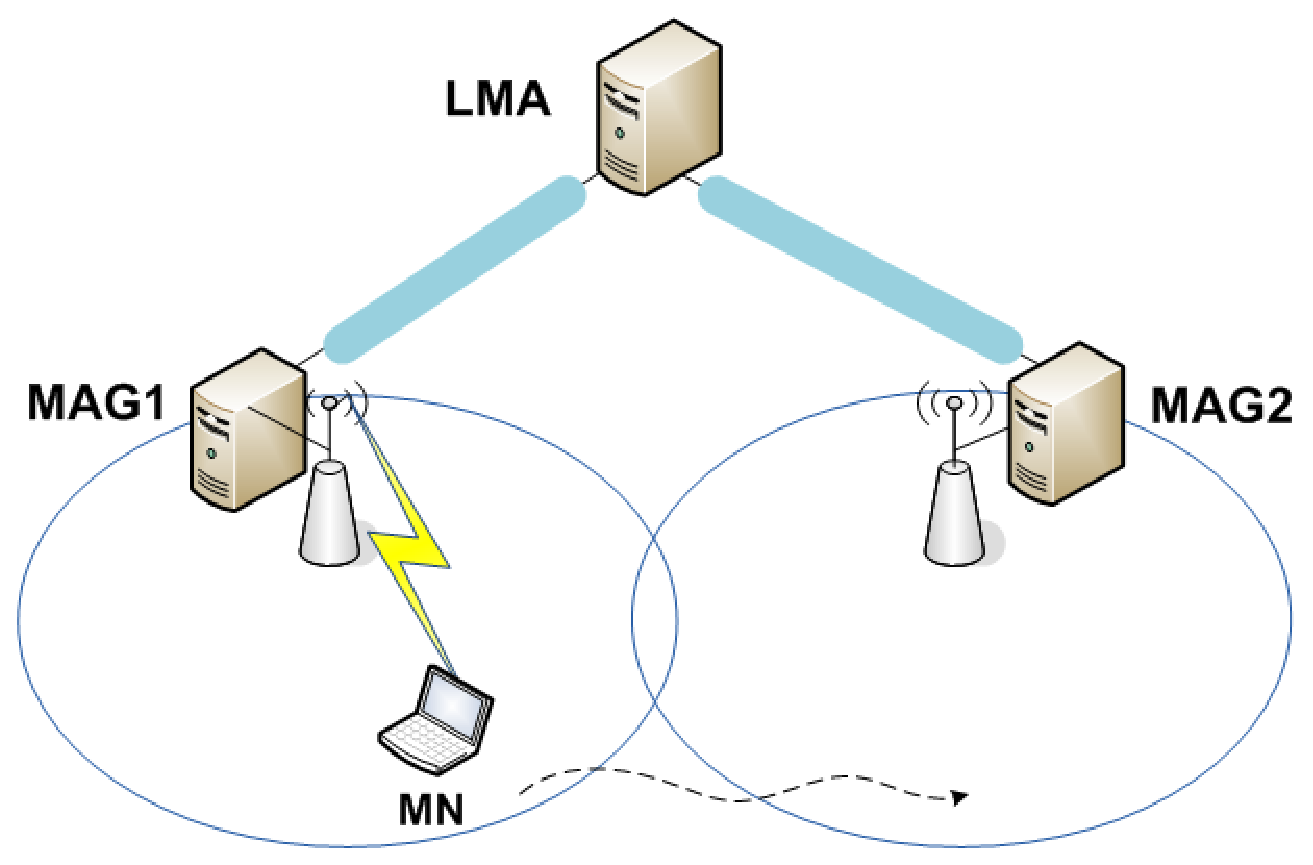
\includegraphics[width=0.50\textwidth]{./Part1/Chapter2/figures/c3_pmip_domain.eps} 
    \caption[The architecture of a PMIPv6 domain]{The architecture of a PMIPv6 domain.}
     \label{fig:c3_pmip_domain}
  \end{center} 
\end{figure}

Compared to MIPv6, PMIPv6 brings some benefits such as: (i) avoiding the complexity of the protocol stack at the MN; (ii) supporting mobility without the MN's involvement; and (iii) reducing tunneling overhead (over the air) and decreasing handover latency \cite{HO_comparison_Lee}.
\begin{figure}[h!] 
 \begin{center} 
 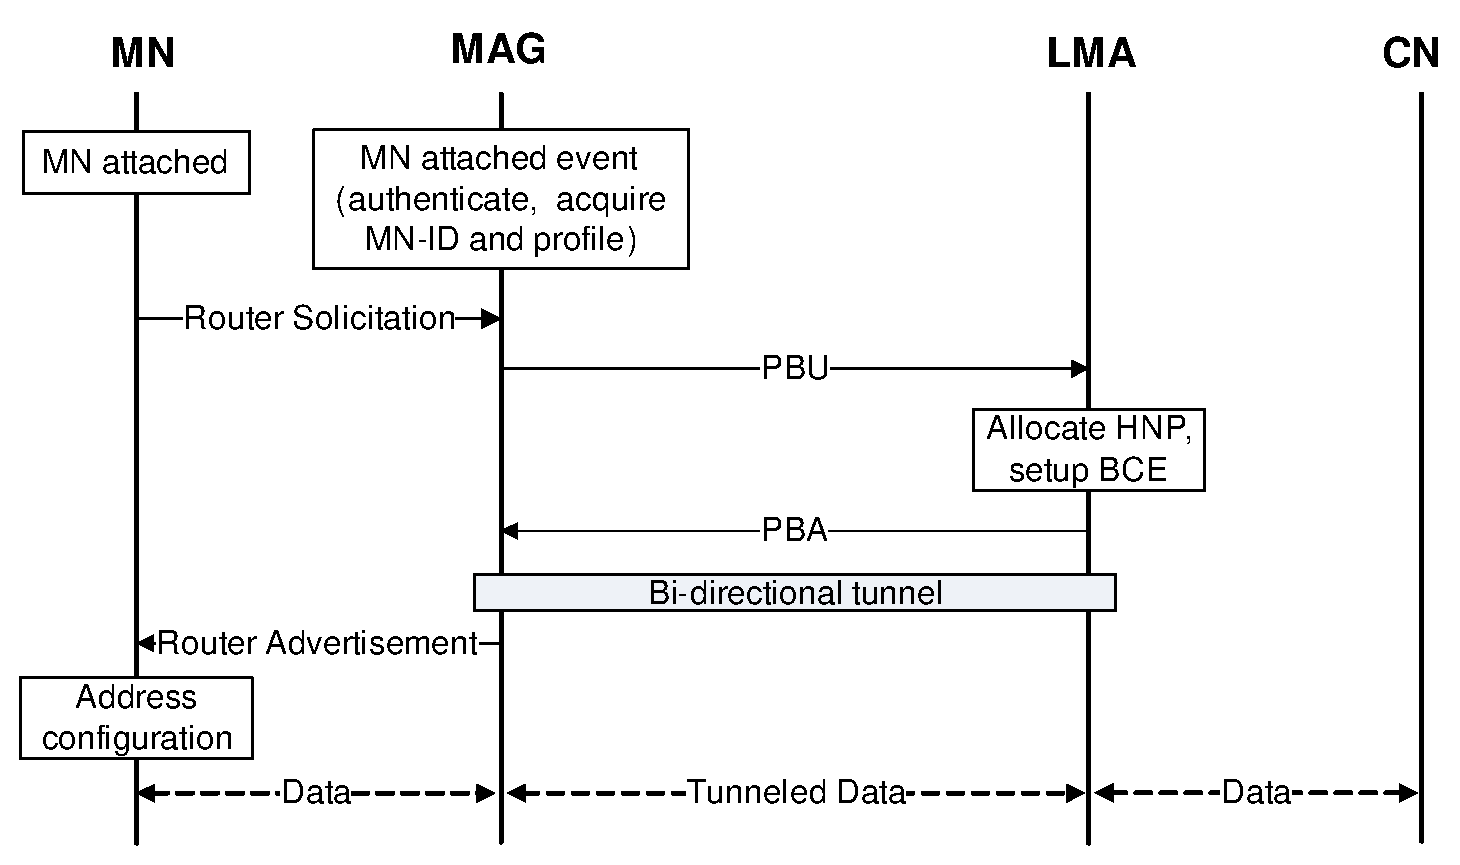
\includegraphics[width=0.60\textwidth]{./Part1/Chapter2/figures/c3_pmip_registration.eps} 
    \caption[Signaling when a mobile node attaches to the PMIPv6 domain]{Signaling when a mobile node attaches to the PMIPv6 domain.}
     \label{fig:c3_pmip_registration}
  \end{center} 
\end{figure}

The operation of PMIPv6 is briefly described as follows. Fig.~\ref{fig:c3_pmip_registration} shows signaling for the MN's initial attachment to a PMIPv6 domain. When an MN enters a PMIPv6 domain (attaches to a MAG), upon the detection of a new MN, the MAG fetches the MN profile, for example from an Authentication, Authorization and Accounting (AAA) server, and verifies if the MN is authorized for the network-based mobility service. Upon a successful authorization, the MAG sends a Proxy Binding Update (PBU) message to LMA to register a new MN. After receiving the PBU message, the LMA allocates a Home Network Prefix (HNP) to the MN, creates a BCE for this MN (including the MN's identifier (MN-ID, for example using the Network Access Identifier (NAI) \cite{NAI}, or its Media Access Control (MAC) address), HNP and the MN's MAG address (Proxy Care-of-Address or Proxy-CoA)). The LMA then replies by a Proxy Binding Acknowledgment (PBA) message including the allocated HNP. The MAG, on receiving the PBA, sets up the forwarding policy for the MN. A bi-directional tunnel is then established between the MAG and the LMA for redirecting the traffic from/to the MN. It is noted that the PBU/PBA messages are based on BU/BA messages with some specific extensions, respectively \cite{PMIPv6}. The MAG then sends a Router Advertisement (RA) message including the allocated HNP to the MN. The MN, based on the HNP, configures its address and can use it to communicate with a corresponding node (CN).
\begin{figure}[h!] 
 \begin{center} 
 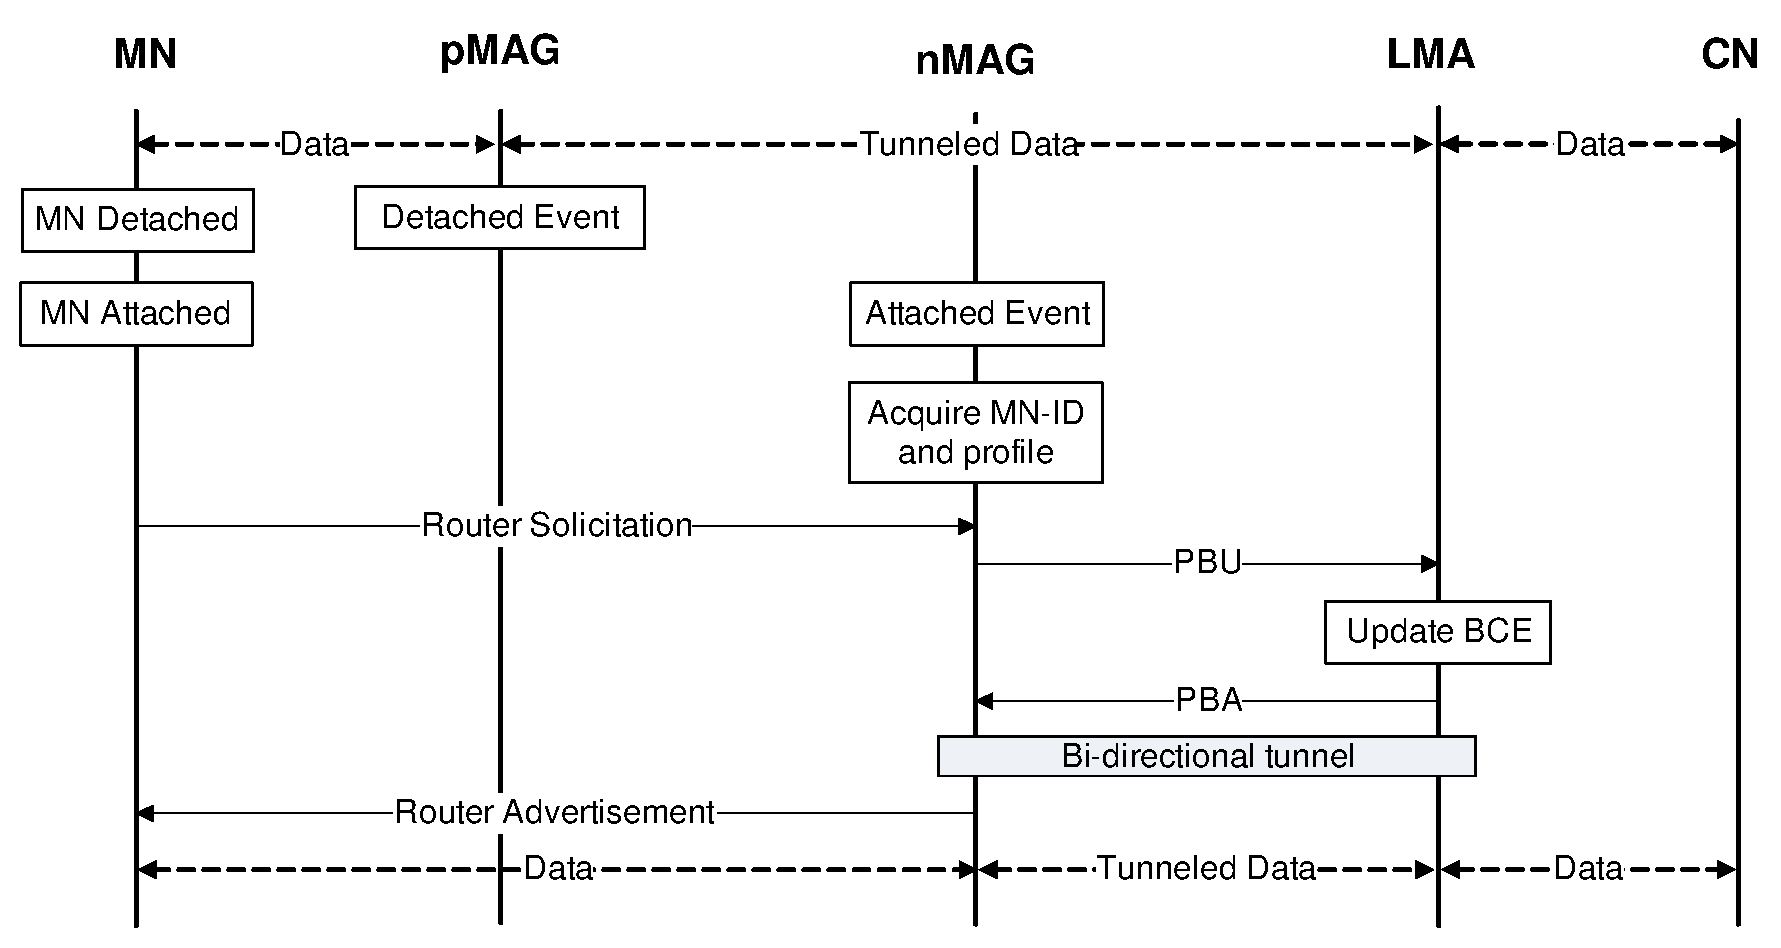
\includegraphics[width=0.68\textwidth]{./Part1/Chapter2/figures/c3_pmip_handover.eps} 
    \caption[Signaling when a mobile node performs a handover in the PMIPv6 domain]{Signaling when a mobile node performs a handover.}
     \label{fig:c3_pmip_handover}
  \end{center} 
\end{figure}

When the MN performs a handover from the previous MAG (pMAG) to a new one (nMAG), the similar process as in the registration step will be executed to update the MN’s current location at the LMA (see Fig.~\ref{fig:c3_pmip_handover}). In this case, the nMAG obtains the same HNP prefix for this MN and can emulate the MN’s home network (through sending RA messages with the same HNP). As a result, the MN is not aware of the mobility and continues to use the same IP address as before. Moreover, the link shared with a given MN of all the MAGs in the domain should be configured with the same link local address to make sure that the MN does not detect link changes as well as avoid the potential address collision issue \cite{PMIPv6} during the handover process.

Similar to FMIPv6, Fast Handovers for PMIPv6 (FPMIPv6) \cite{FPMIPv6} provides a fast handover mechanism for PMIPv6 in order to minimize the handover latency and the packet loss. Again, a bi-directional tunnel is established between the previous MAG and the current one to forward the packets to/from the MN. Also, the MN should provide information about the target network to the pMAG through L2 signaling. However, it inherits potential risks of erroneous movement and out-of-order packets delivery problem from FMIPv6

\paragraph{Extensions to PMIPv6}
Typically, the performance of a mobility management protocol is measured using such well-known metrics as signaling cost, handover latency, and packet loss. The signaling cost consists of the location update cost and the packet delivery cost. Handover latency is defined as the total time needed to complete the handover procedures. During this time, the MN cannot send or receive any packets. The handover latency typically consists of layer 2 handover duration and layer 3 one. The packet loss is the amount of lost packets originated from or sent to an MN during its handover. 

Various papers have been proposed which aim at improving PMIPv6 in terms of handover latency and signaling cost. In \cite{pmip_paging_Hong, pmip_paging_Lee}, the authors applied the paging technologies to PMIPv6 to reduce the location update signaling cost for the mobile host in the idle mode. In \cite{pmip_handover_latency_Kang}, the authors used the Neighbor Discovery (ND) message of IPv6 to reduce the handover latency and packet buffering at the MAG. In this case, the pMAG sent the MN's profile to the neighbor MAGs through ND message. Similarly, in \cite{pmip_handover_latency_Kim}, the pMAG sent the MN’s HNP to the adjacent MAGs in advance in order to perform the address configuration quickly after MN’s handover. In \cite{pmip_handover_latency_Magagula}, the improvement on handover latency was achieved by using the IEEE 802.21 Media Independent Handover services. 

Similar to in MIPv6, in \cite{RO_pmip_Krishnan, RO_pmip_Rasem}, different route optimization schemes for PMIPv6 were also considered. Thus, the traffic could be routed in a better route bypassing the LMA. Unlike MIPv6, one of the main drawbacks of PMIPv6 is that the inter-domain handover is not supported. Thus, inter-domain mobility support in PMIPv6 has been proposed in \cite{inter_pmip_Giaratta,inter_pmip_Neumann, inter_pmip_Ma,Thinh_WCNC_DMM}. 

\subsubsection{Mobility Management in the Current Cellular Networks}
\begin{figure}[h!] 
 \begin{center} 
 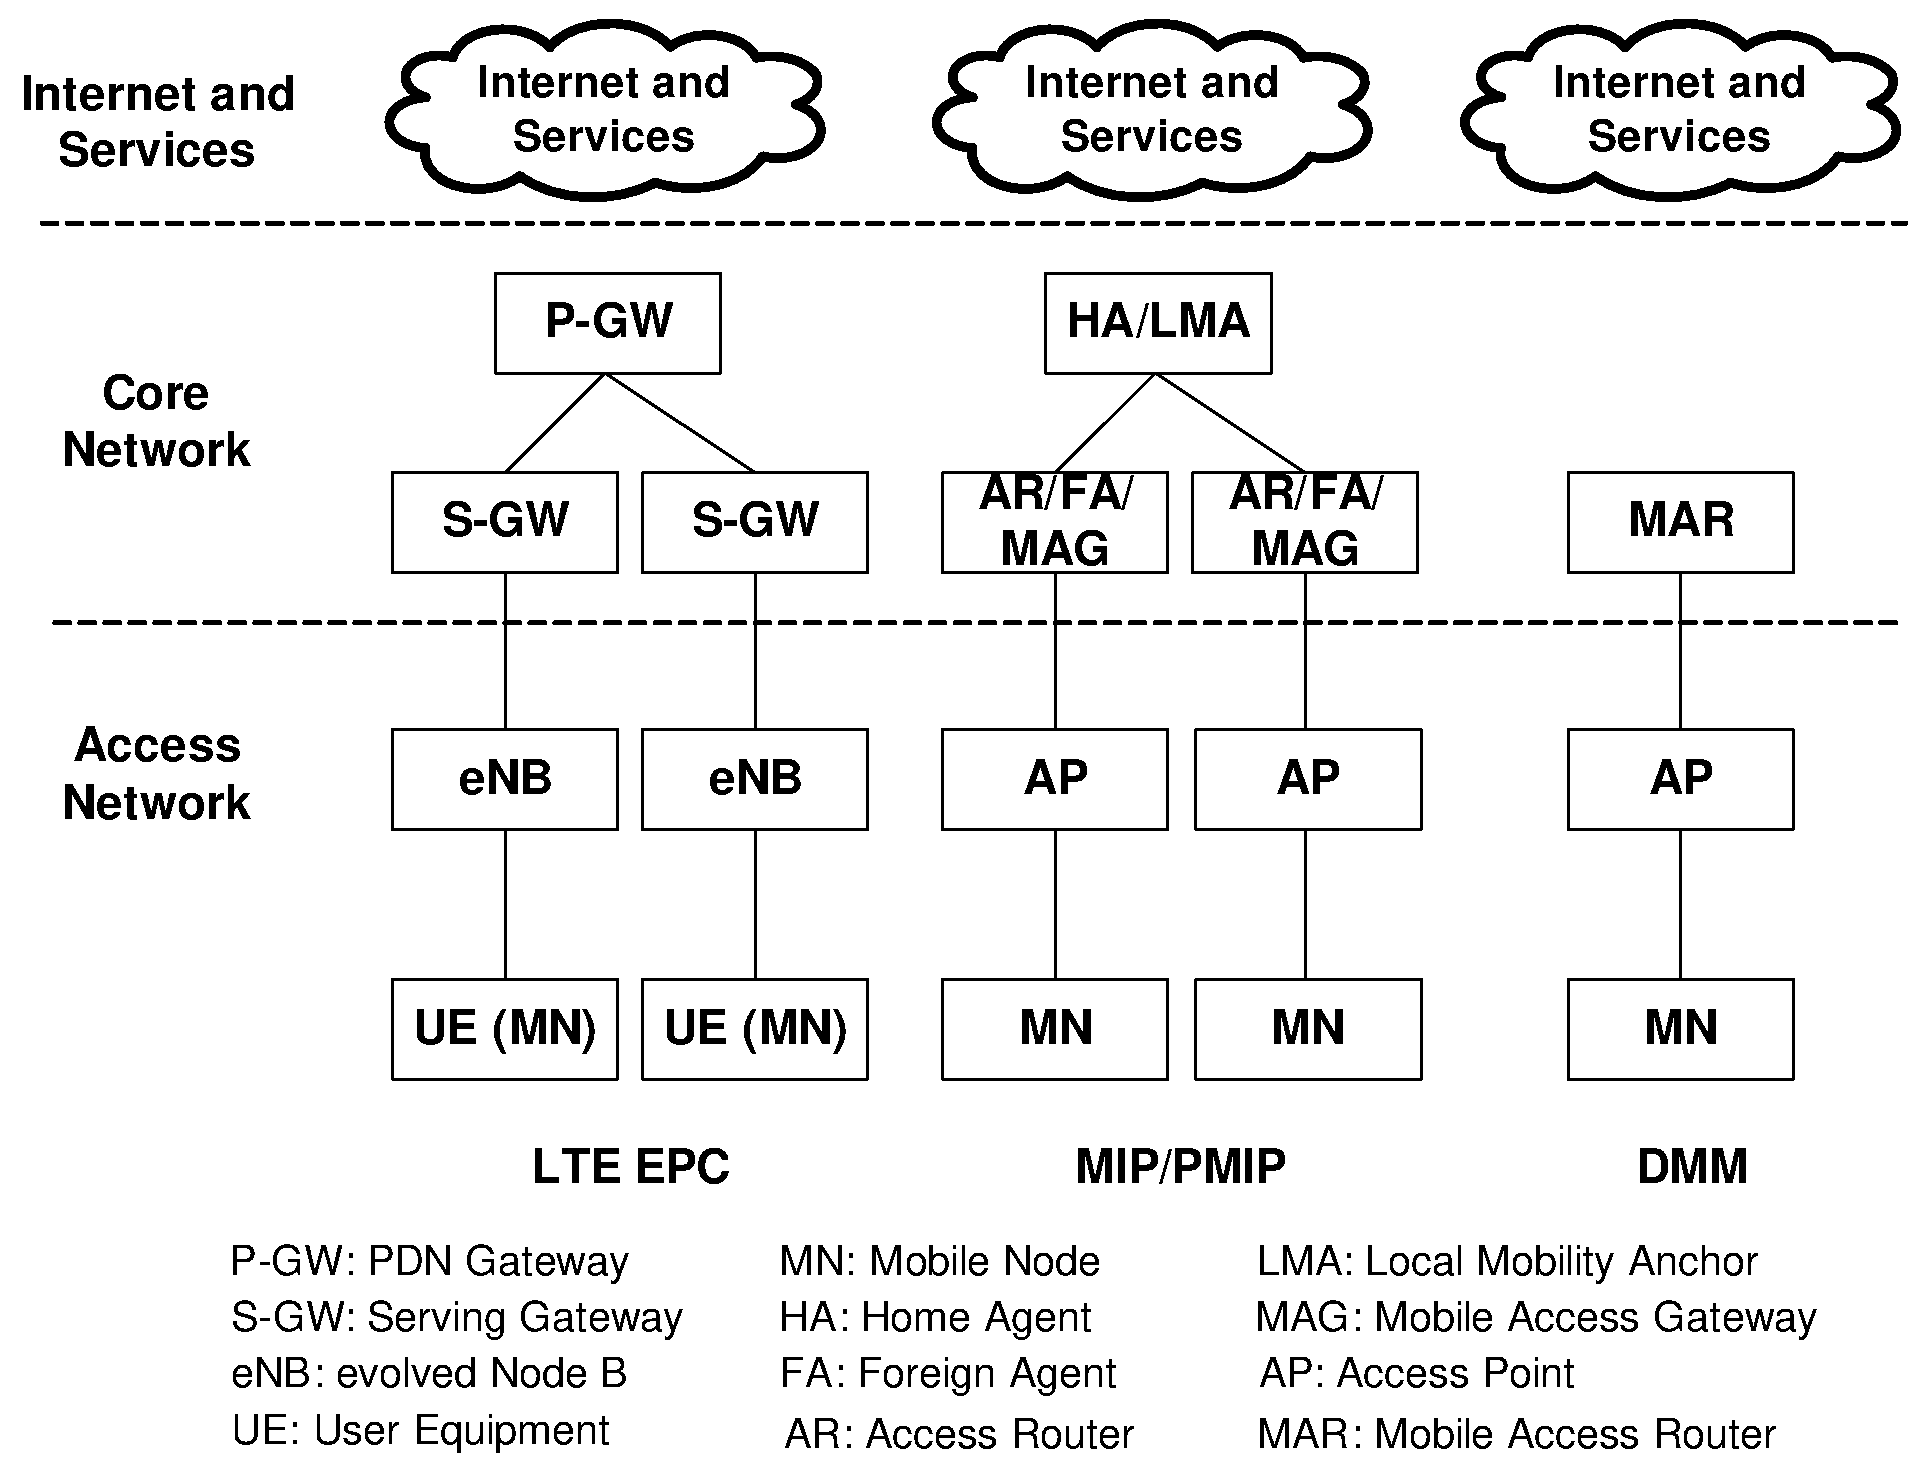
\includegraphics[width=0.70\textwidth]{./Part1/Chapter2/figures/c3_network_level.eps} 
    \caption{Mobile network architecture.}
     \label{fig:c3_network_level}
  \end{center} 
\end{figure}

The current mobile network architecture is highly centralized and hierarchical \cite{DMM_Bertin}. Following the hierarchical architecture, the network elements can be placed into three levels: Internet and services, core network, and access network. For example, the 3GPP cellular network consists of SGSN (Serving GPRS Support Node) and GGSN (Gateway GPRS Support Node). The evolved packet core (EPC) network \cite{3gpp.23.002} includes a packet data network gateway (P-GW), serving gateway (S-GW), and evolved Node B (eNB) as shown in the leftmost of Fig.~\ref{fig:c3_network_level}. Thus IP mobility protocols, such as PMIPv6 and DSMIPv6, which have been adopted as IP mobility protocols for the 3GPP EPC architecture, are inline with the centralized and hierarchical of the network architecture. 

Following the hierarchical architecture, the centralized mobility management protocols rely on the mobility anchor (HA in MIPv6 and LMA in PMIPv6) to enable the mobility support. Therefore, both the mobile context and traffic encapsulation need to be maintained at the mobility anchor. The number of mobile devices and their traffic demand increases exponentially make the centralized mobility management solutions encounter several problems and limitations as stated in \cite{DMM_issues,DMM_problem_statement}. Among them, we just highlight the following issues:

\begin{itemize}
\item \textit{Sub-optimal routing and end-to-end delay}: Since the data traffic always traverses the central mobility anchor, it often results in a longer route, especially when the CN and the MN are close to each other but far from the anchor. The same thing happens in case of Content Delivery Networks (CDN), in which the content providers place their data to the edge of the network. As a result, the end-to-end delay will be increased. 
\item \textit{Scalability problem}: Maintaining MN's context and processing the packets from/to the MN usually require resources of the mobility anchor as well as the networks (require more bandwidth of the links close to the mobility anchor), thus reducing the scalability of the system.  
\item \textit{Resource waste}: The mobility service is always provided even for the sessions that do not require the mobility management support e.g., the sessions which launch and complete while the node is connected to the same layer 3 point of attachment, or the sessions which can handle mobility at the application layer e.g.,  SIP-based sessions. Thus, by providing mobility support for the MN/service when it is really needed, the network resource (e.g., reducing signaling load) can be saved.   
\item \textit{Reliability}: The central mobility anchor in general poses a bottleneck and single point of failure.  
\end{itemize}

\subsection{Distributed Mobility Management}
As stated in the previous section, the mobile network is currently evolving towards the flat architecture. To cope with this evolution, distributed mobility management (DMM) solutions have been proposed. DMM concept aims at addressing the limitations of the centralized mobility approach (e.g., bottleneck and single point of failure, etc.) raised when a large number of mobile devices and data traffic are considered in a flat architecture \cite{DMM_issues,DMM_problem_statement}. DMM is currently a hot topic which gains much interest from both the academia and the industry. The IETF has recently chartered the Distributed Mobility Management (DMM) working group\footnote{IETF DMM WG: https://ietf.org/wg/dmm/charter/} which specifies the solutions allowing for setting up IP networks supporting a distributed anchoring model. The key concepts of DMM are: i) the mobility is distributed among network entities and placed as close as possible to the MN e.g., at the router edge of the access network; and ii) the mobility management is dynamically provided for the sessions that really require service continuity. 

Following the DMM requirement (REQ4) in terms of reusing/extending the existing IETF IP mobility protocols (i.e., MIPv6 and PMIPv6, and so on), the existing proposals (e.g., \cite{DMA, PMIP_based_DMM_Bernardos}) aim at making these solutions work in a distributed manner by deploying multiple mobility anchors (HA in MIPv6 and LMA in PMIPv6) at the edge of the access network, serving as the default gateway of the mobile node. From the IETF point of view, there are two main groups of solutions: the host-based and the network-based. The host-based approach provides a global (as well as a local) mobility support for the MNs while the network-based provides a local mobility support for the MNs moving in a single domain. 
\subsubsection{DMM from IETF Point of View}
\paragraph{Host-based DMM Approach}

The terminology used by this subsection names an access router that provides the host-based DMM mobility support is a Host-based Mobile Access Router (HMAR). The HMAR, similar to HA, is a mobility anchor which allocates a network prefix to the MN and maintains the binding cache for its registered MNs. The current HMAR (cHMAR) is the one to which the MN is currently attached, while the anchor HMAR (aHMAR) of an address/session is the one where the prefix in use is allocated (and the session is initiated using this address as the source address).  

In the host-based approach, the MN is required to participate to the signaling process. There are two main schemes for the host-based approach. In the first scheme, the tunneling for the handover session is established between the anchor HMAR and the MN as similar to the MIPv6 protocol. In the second scheme, the tunnel is established between the current HMAR and the anchor one. 

Regarding the first host-based DMM scheme as proposed in \cite{MIP_based_DMM_Bernardos,MIP_based_DMM_Hassan}, whenever an MN attaches to a HMAR it gets an IPv6 address. The cHMAR plays the role of HA for the address allocated at its network. While attaching to the cHMAR, the MN can start new communications (flows) with the CNs using the current address as the source address of the flows. These new flows are then routed in a standard way without the tunneling mechanism. When the MN performs a handover, if these ongoing flows are still alive, these flows are routed via the routers where the flows were originally initiated (aHMAR) using the tunneling mechanism. Thus, the MN needs to register its current topological location to each aHMAR (corresponding to each active HoA in use) by means of BU/BA messages. In this case, the current HoA actually plays the role of CoA. A bi-directional tunnel is then established between each aHMAR and the MN. Thus, the traffic passes through the mobility anchor via the bi-directional tunnel. Fig.~\ref{fig:c3_mip_dmm} and Fig.~\ref{fig:c3_mip_dmm_signaling} represent an example scenario of host-based DMM support.

It is noted that the MN should perform a location update process for each active IP address. As a result, it requires the MN to manage the list of active HoAs and the associated aHMARs, as well as the list of active sessions using the corresponding HoA. Moreover, the MN needs an additional mechanism which allows to select the right IP address to use for each session. The binding cache of the HMARs and the list of active sessions of the MN are illustrated in Fig.\ref{fig:c3_mip_dmm_b}.
\begin{figure}[h!]
\centering
\subfloat[]{\includegraphics[width=0.47\textwidth]{./Part1/Chapter2/figures/c3_mip_dmm.eps} \label{fig:c3_mip_dmm_a}}\,\,\,\,\,\,
\subfloat[]{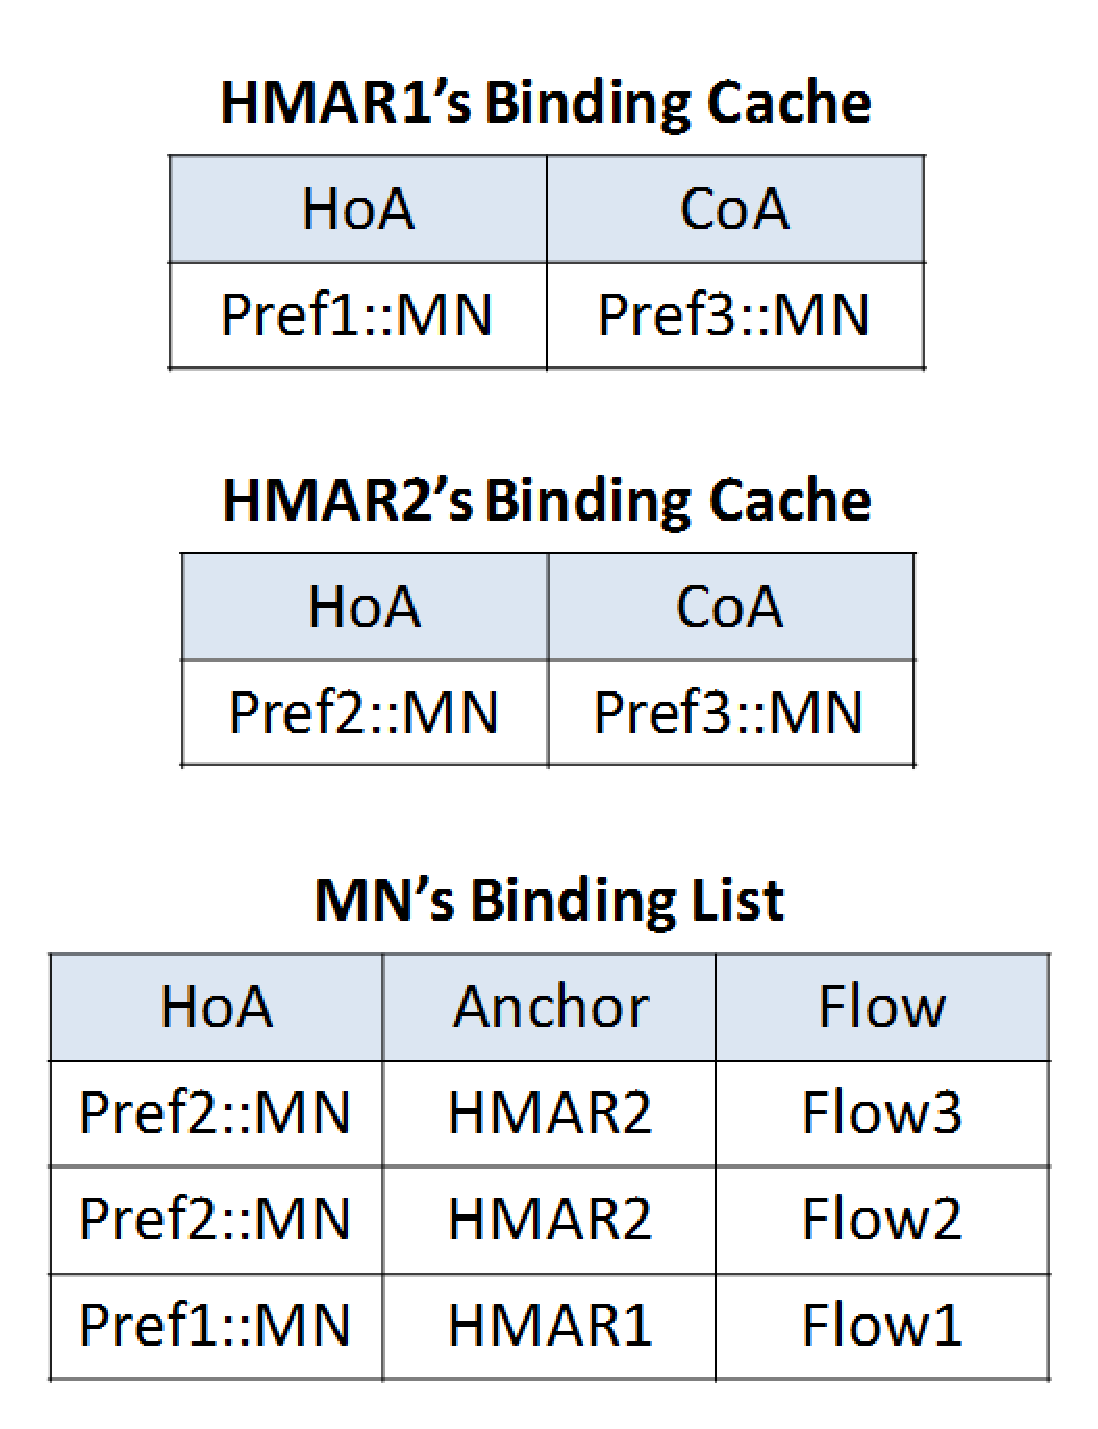
\includegraphics[width=0.33\textwidth]{./Part1/Chapter2/figures/c3_mip_dmm_b.eps}\label{fig:c3_mip_dmm_b}}
\caption[Mobility management in the host-based approach (scheme 1).]{Mobility management in the host-based approach (scheme 1): (a) Operation description. (b) Binding cache.}
\label{fig:c3_mip_dmm}
\end{figure}
\begin{figure}[h!] 
 \begin{center} 
 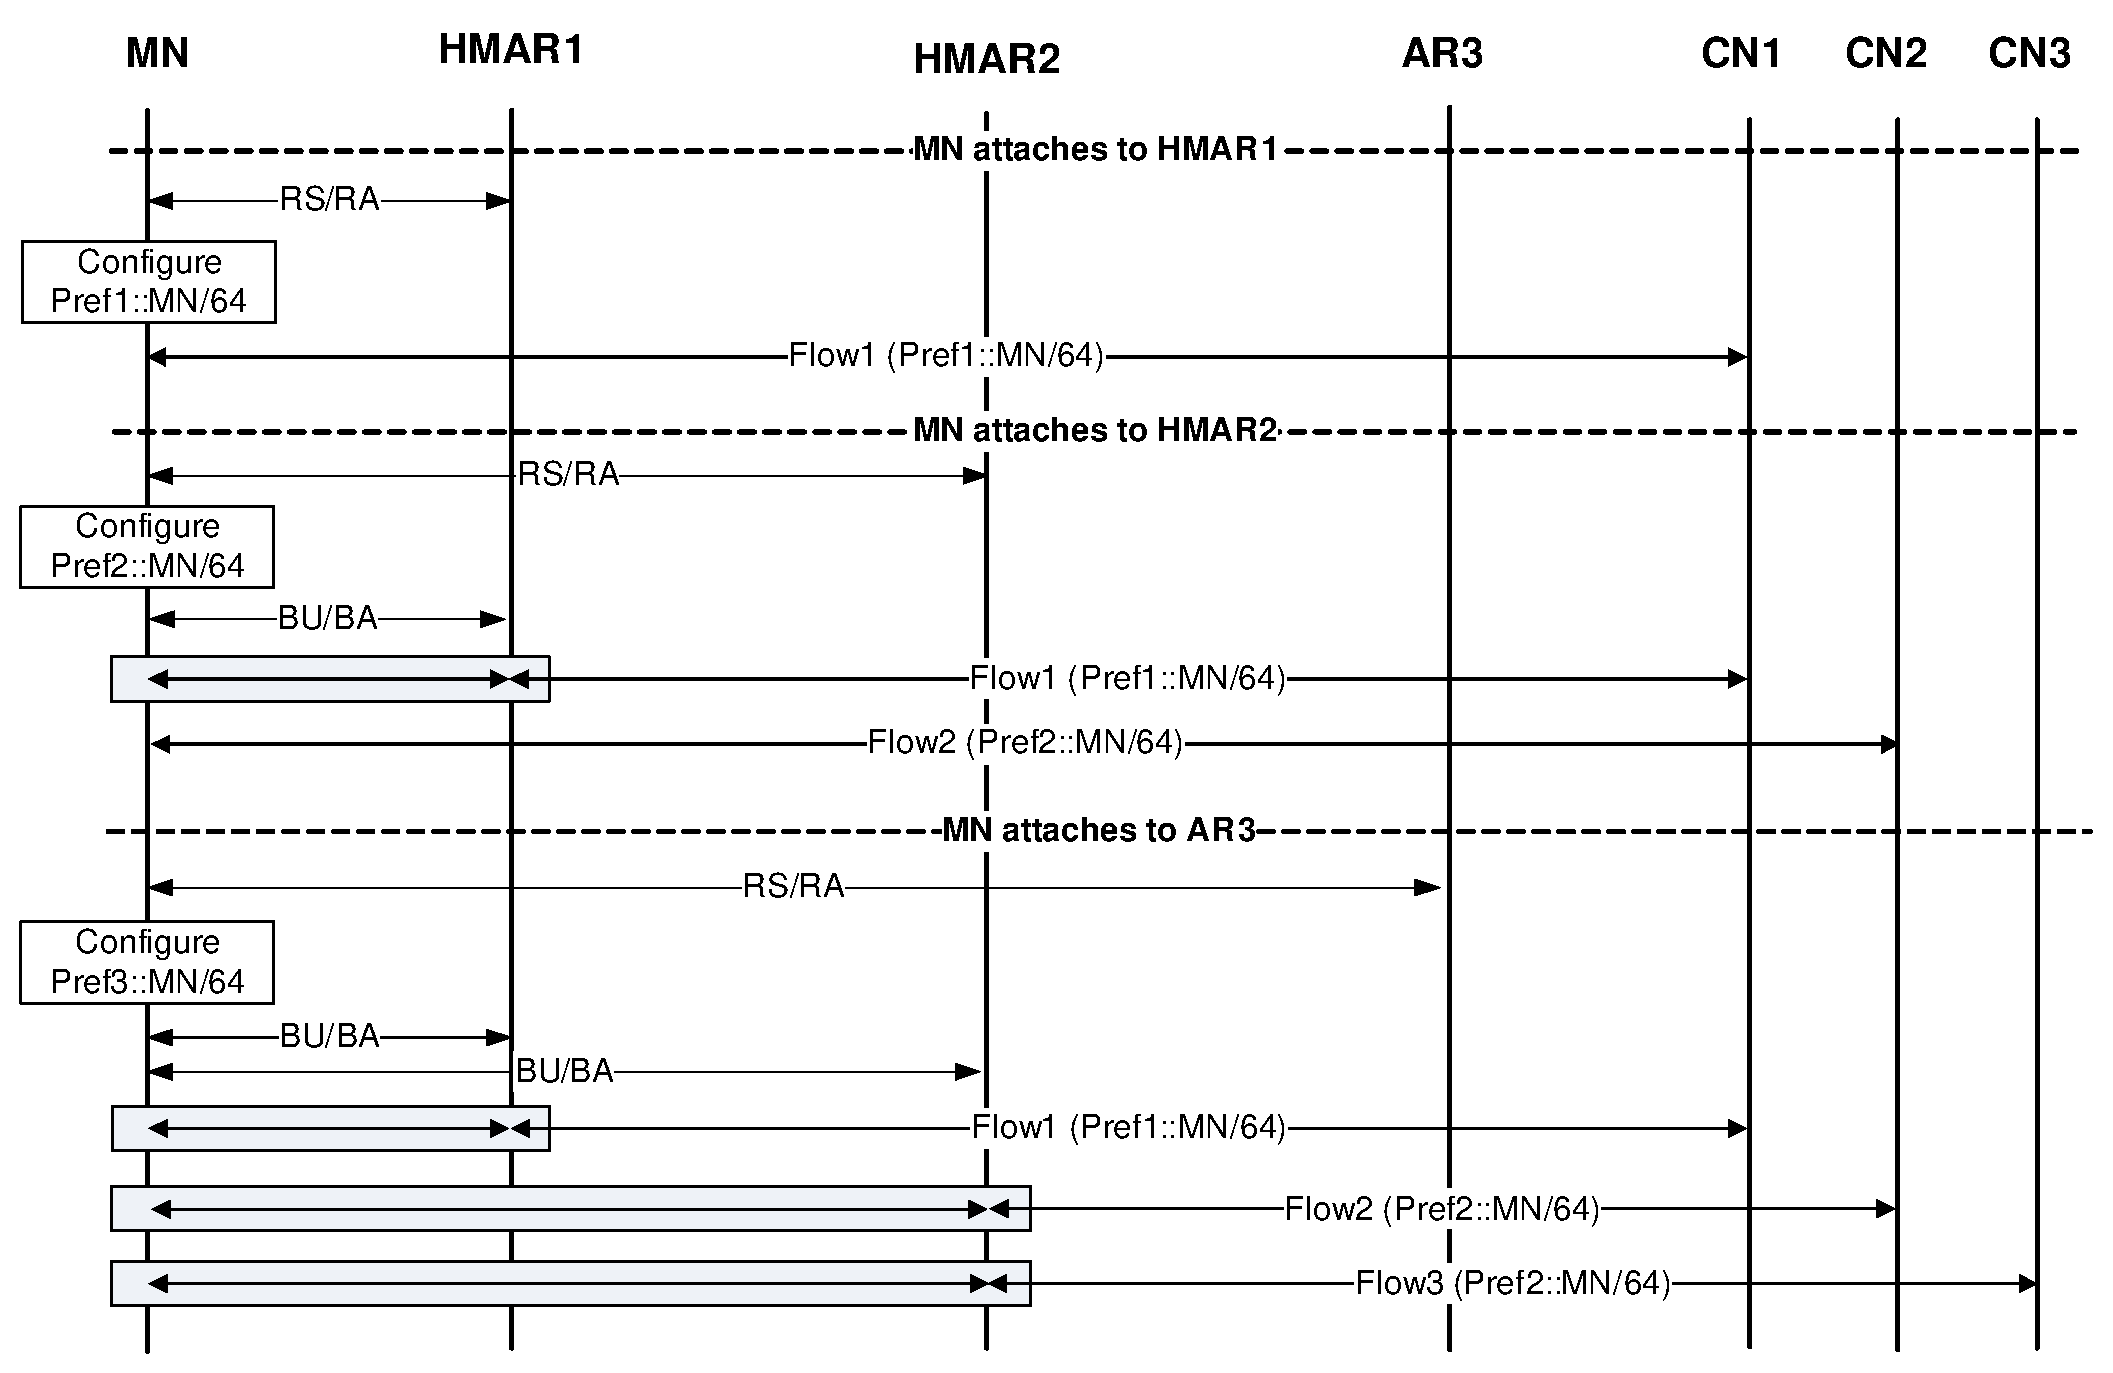
\includegraphics[width=0.9\textwidth]{./Part1/Chapter2/figures/c3_mip_dmm_signaling.eps} 
    \caption{Signaling for the mobility management in the host-based approach (scheme 1).}
     \label{fig:c3_mip_dmm_signaling}
  \end{center} 
\end{figure}

Additionally, as a global mobility, another scenario should be taken into account in which the MN moves to a typical access router's area (without supporting the host-based DMM) as discussed in \cite{DMM_analysis_Hassan, MIP_based_DMM_Condeixa}. In this circumstance, the MN should select one among the active IP addresses to be served as the source address, and the associated aHMAR as the HA. The MN then performs the normal MIPv6 operation. For example, as shown in Fig.\ref{fig:c3_mip_dmm}, the MN attaches to a typical access router (AR3). After getting a prefix (Prefix3::/64), the MN configures its IP address (Pref3::MN/64). When the MN starts a new session (Flow3), it selects HoA2 and HMAR2 as the source address and the corresponding HA, respectively. As a result, the Flow3 is routed via the tunnel HMAR2-MN. Regarding the ongoing flows, the Flow1 and Flow2 are then routed via HMAR1 and HMAR2 using the tunnel HMAR1-MN and HMAR2-MN, respectively.

As stated earlier, the MN needs to inform all active aHMARs about its current location by means of BU/BA messages. Thus, the mobility signaling cost (over the air) is relatively high. As a result, the second host-based DMM scheme is proposed in order to reduce the mobility signaling cost of the MN (see Fig.\ref{fig:c3_mip_dmm_2}). In this case, the MN only needs to exchange the BU/BA messages with the current mobility anchor \cite{DMM_IETF_Lee}. The BU includes the MN's prefixes in use and the corresponding aHMAR. Based on this information, the BU/BA messages are exchanged between the cHMAR and each aHMAR which allows establishing the tunnel between them. The active sessions are then routed via the corresponding aHMAR utilizing the tunneling mechanism. Again, if the MN moves to a typical AR's area, the tunnel is established between the MN and the aHMAR as similar to the previous host-based scheme.  
\begin{figure}[h!]
\centering
\subfloat[]{\includegraphics[width=0.47\textwidth]{./Part1/Chapter2/figures/c3_mip_dmm_2.eps} \label{fig:c3_mip_dmm_2_a}}\,\,\,\,\,\,
\subfloat[]{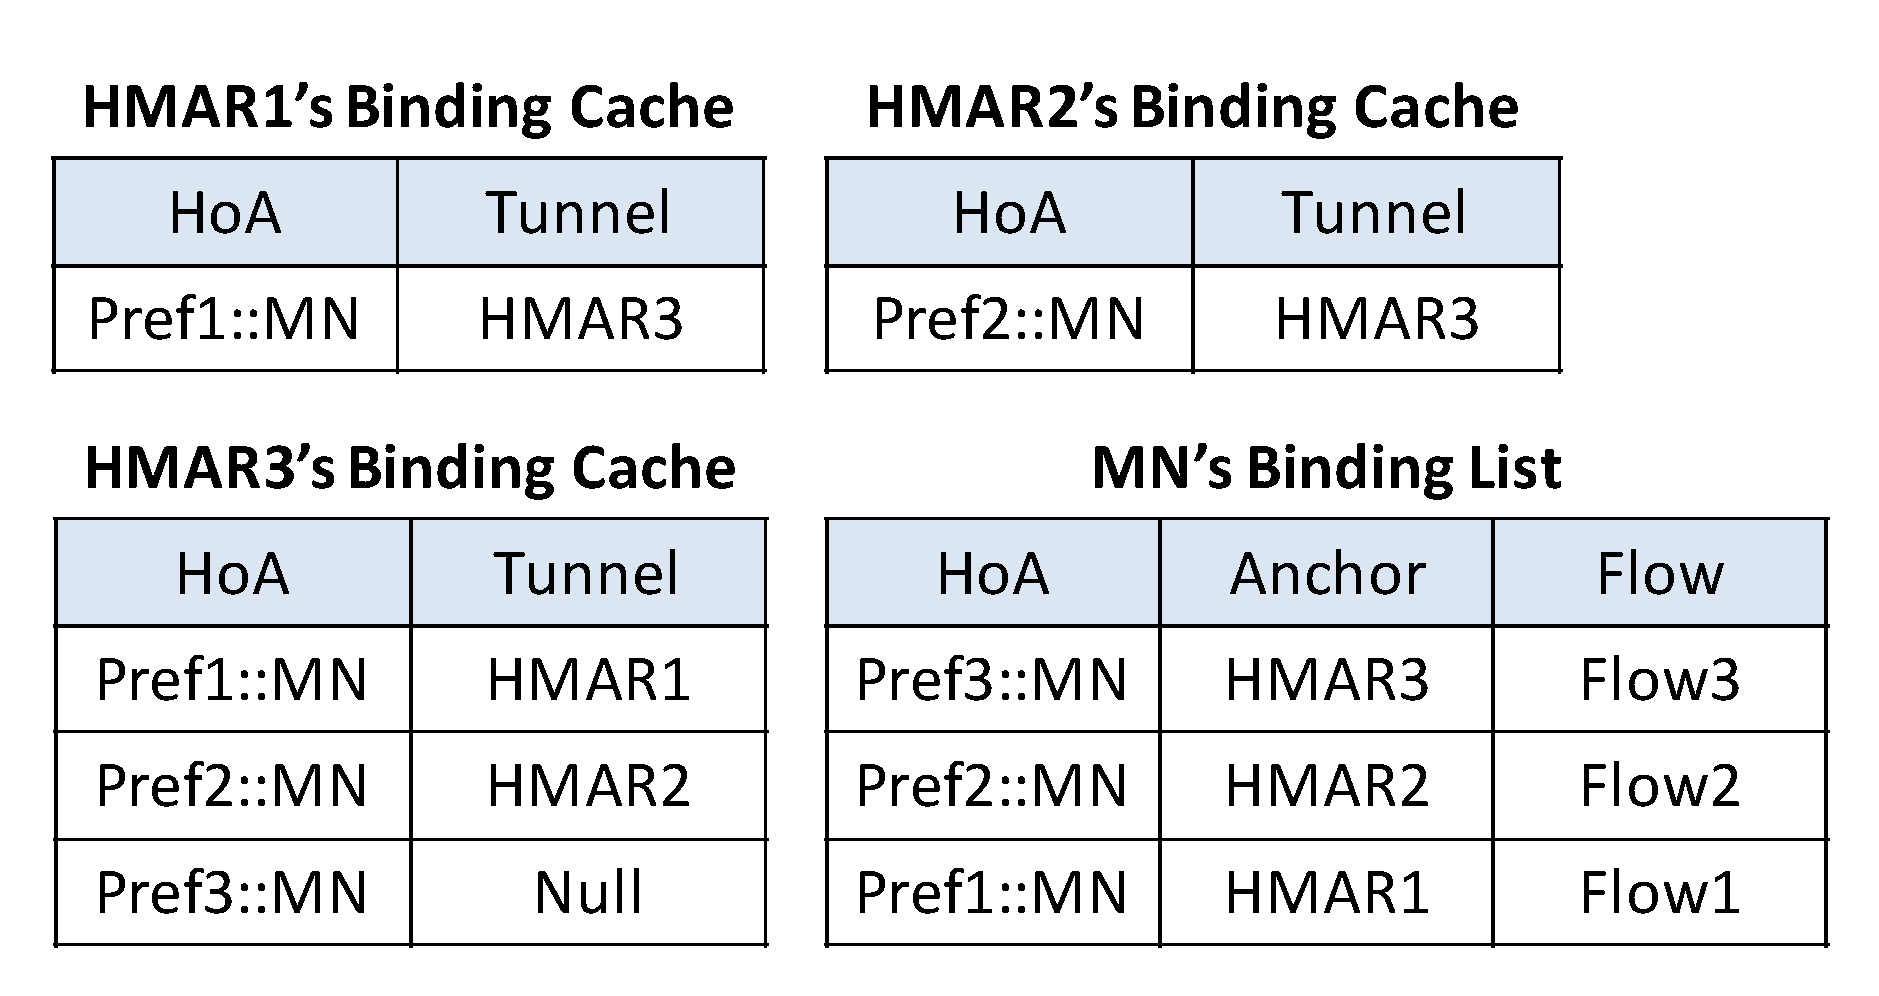
\includegraphics[width=0.47\textwidth]{./Part1/Chapter2/figures/c3_mip_dmm_2_b.eps}\label{fig:c3_mip_dmm_2_b}}
\caption[Mobility management in the host-based approach (scheme 2).]{Mobility management in the host-based approach (scheme 2): (a) Operation description. (b) Binding cache.}
\label{fig:c3_mip_dmm_2}
\end{figure}

It is important to note that the MN keeps the information of the active HoAs and their associated aHMAR when having at least one active session using this HoA. Otherwise, the information will be deleted. Thus, in this thesis, we suggest that at least one HoA should be considered as a global address and should be kept throughout its lifetime e.g., an address allocated at the MN's typical location. 

\paragraph{Network-based DMM approach}
Unlike the host-based DMM, the network-based approach does not require the MN to participate in the mobility signaling process. To do so, a new network entity, namely Network-based DMM Access Router (NMAR) is introduced. The NMAR is an access router supporting the network-based DMM mobility. The NMAR thus performs both LMA's and MAG's functionality. Acting as a MAG, the NMAR detects the attachment of the MN, while as an LMA it allocates a HNP to the MN. Again, we introduce two logical NMARs: i) a current NMAR (cNMAR) is the NMAR to which the MN is currently attached; and ii) an anchor NMAR (aNMAR) is the NMAR to which the MN's HNP is allocated (the session is initiated). 

Similar to the host-based DMM, when an MN attaches to a NMAR, it obtains an IPv6 address. Typically, it uses the current IP address to start new sessions. The data traffic is routed using the normal IP routing without any tunneling mechanism. If the MN performs a handover and some sessions are still alive (namely handover sessions), the mobility management procedure is activated as follows. The cNMAR, acting as the MAG, exchanges PBU/PBA messages with the aNMAR which acts as the LMA of the flows initiated at the aNMAR. Once the PBU/PBA signaling is completed, a tunnel is established between the cNMAR and the aNMAR for the sessions initiated at the aNMAR. However, an important question raised is that how the nNMAR learn about the addresses of the aNMARs. 
\begin{figure}[h!]
\centering
\subfloat[]{\includegraphics[width=0.50\textwidth]{./Part1/Chapter2/figures/c3_pmip_dmm.eps} \label{fig:c3_pmip_dmm_a}}\,\,\,\,\,\,
\subfloat[]{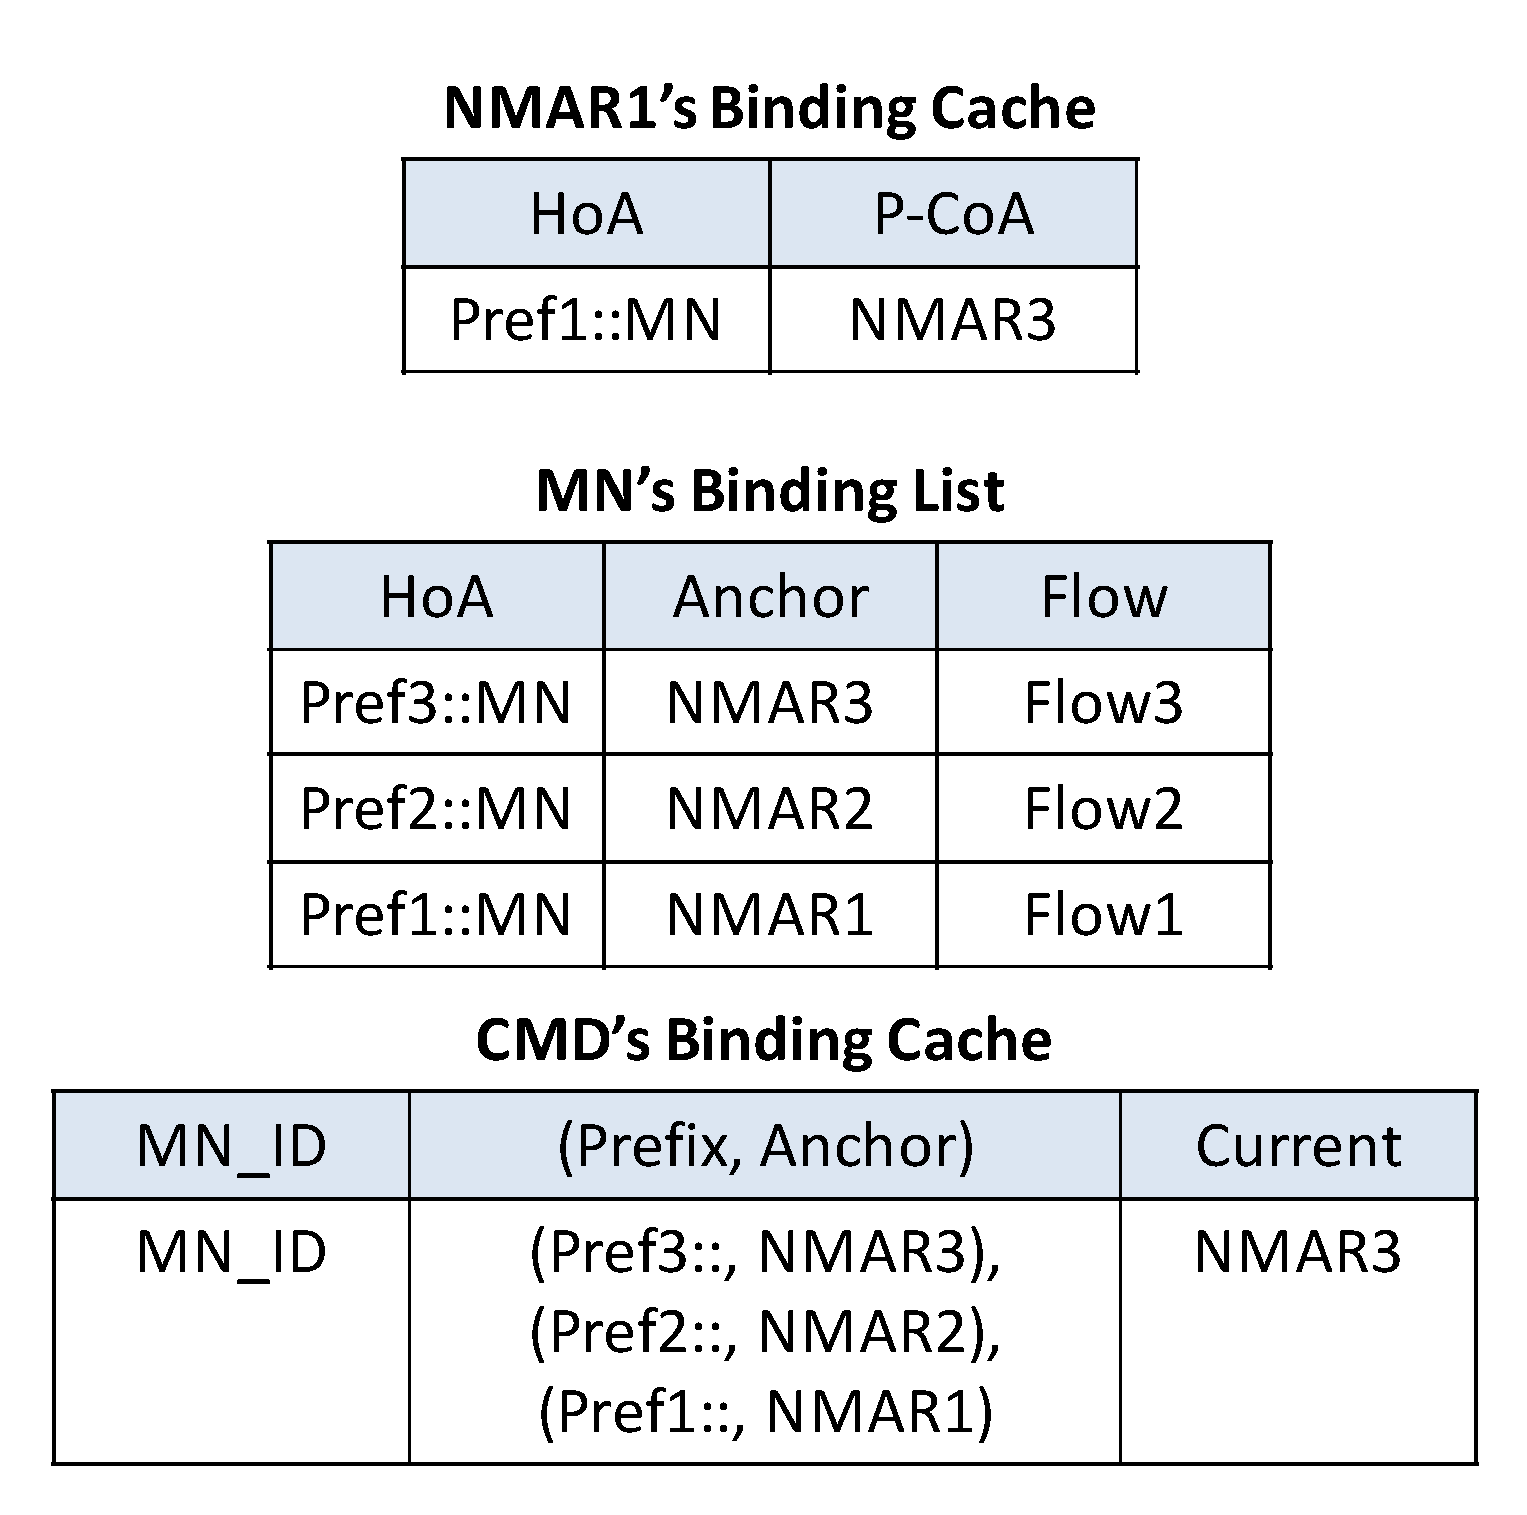
\includegraphics[width=0.39\textwidth]{./Part1/Chapter2/figures/c3_pmip_dmm_b.eps}\label{fig:c3_pmip_dmm_b}}
\caption[Mobility management in the network-based approach.]{Mobility management in the PMIP-based approach: (a) Operation description. (b) Binding cache.}
\label{fig:c3_pmip_dmm}
\end{figure}

There is several mechanisms allowing the nNMAR to know the address of the aNMARs. The first method \cite{DMA} relies on a centralized database (namely centralized mobility database, or CMD) which stores the mobility-related information of each MN in the domain such as the list of MN's HoAs, the associated aNMARs' address as similar to in \cite{inter_domain_DMM}. Although it ensures that the mobility process is totally transparent to the MN, this mechanism introduces again a centralized anchor, however, for control plane only. The data plane is still fully distributed among the network entities. That is the reason why this scheme is considered as a partially distributed scheme. The second method relies on the information provided by the MN as specified in \cite{PMIP_based_DMM_Giust}. In other words, the NMAR retrieves the address of the anchor NMARs from the MN. As a result, the MN is no longer transparent to the mobility process. Therefore, in some papers \cite{DMM_analysis_Hassan, DMM_IETF_Lee} this method is considered as a host-based scheme as stated above. 
\begin{figure}[h!] 
 \begin{center} 
 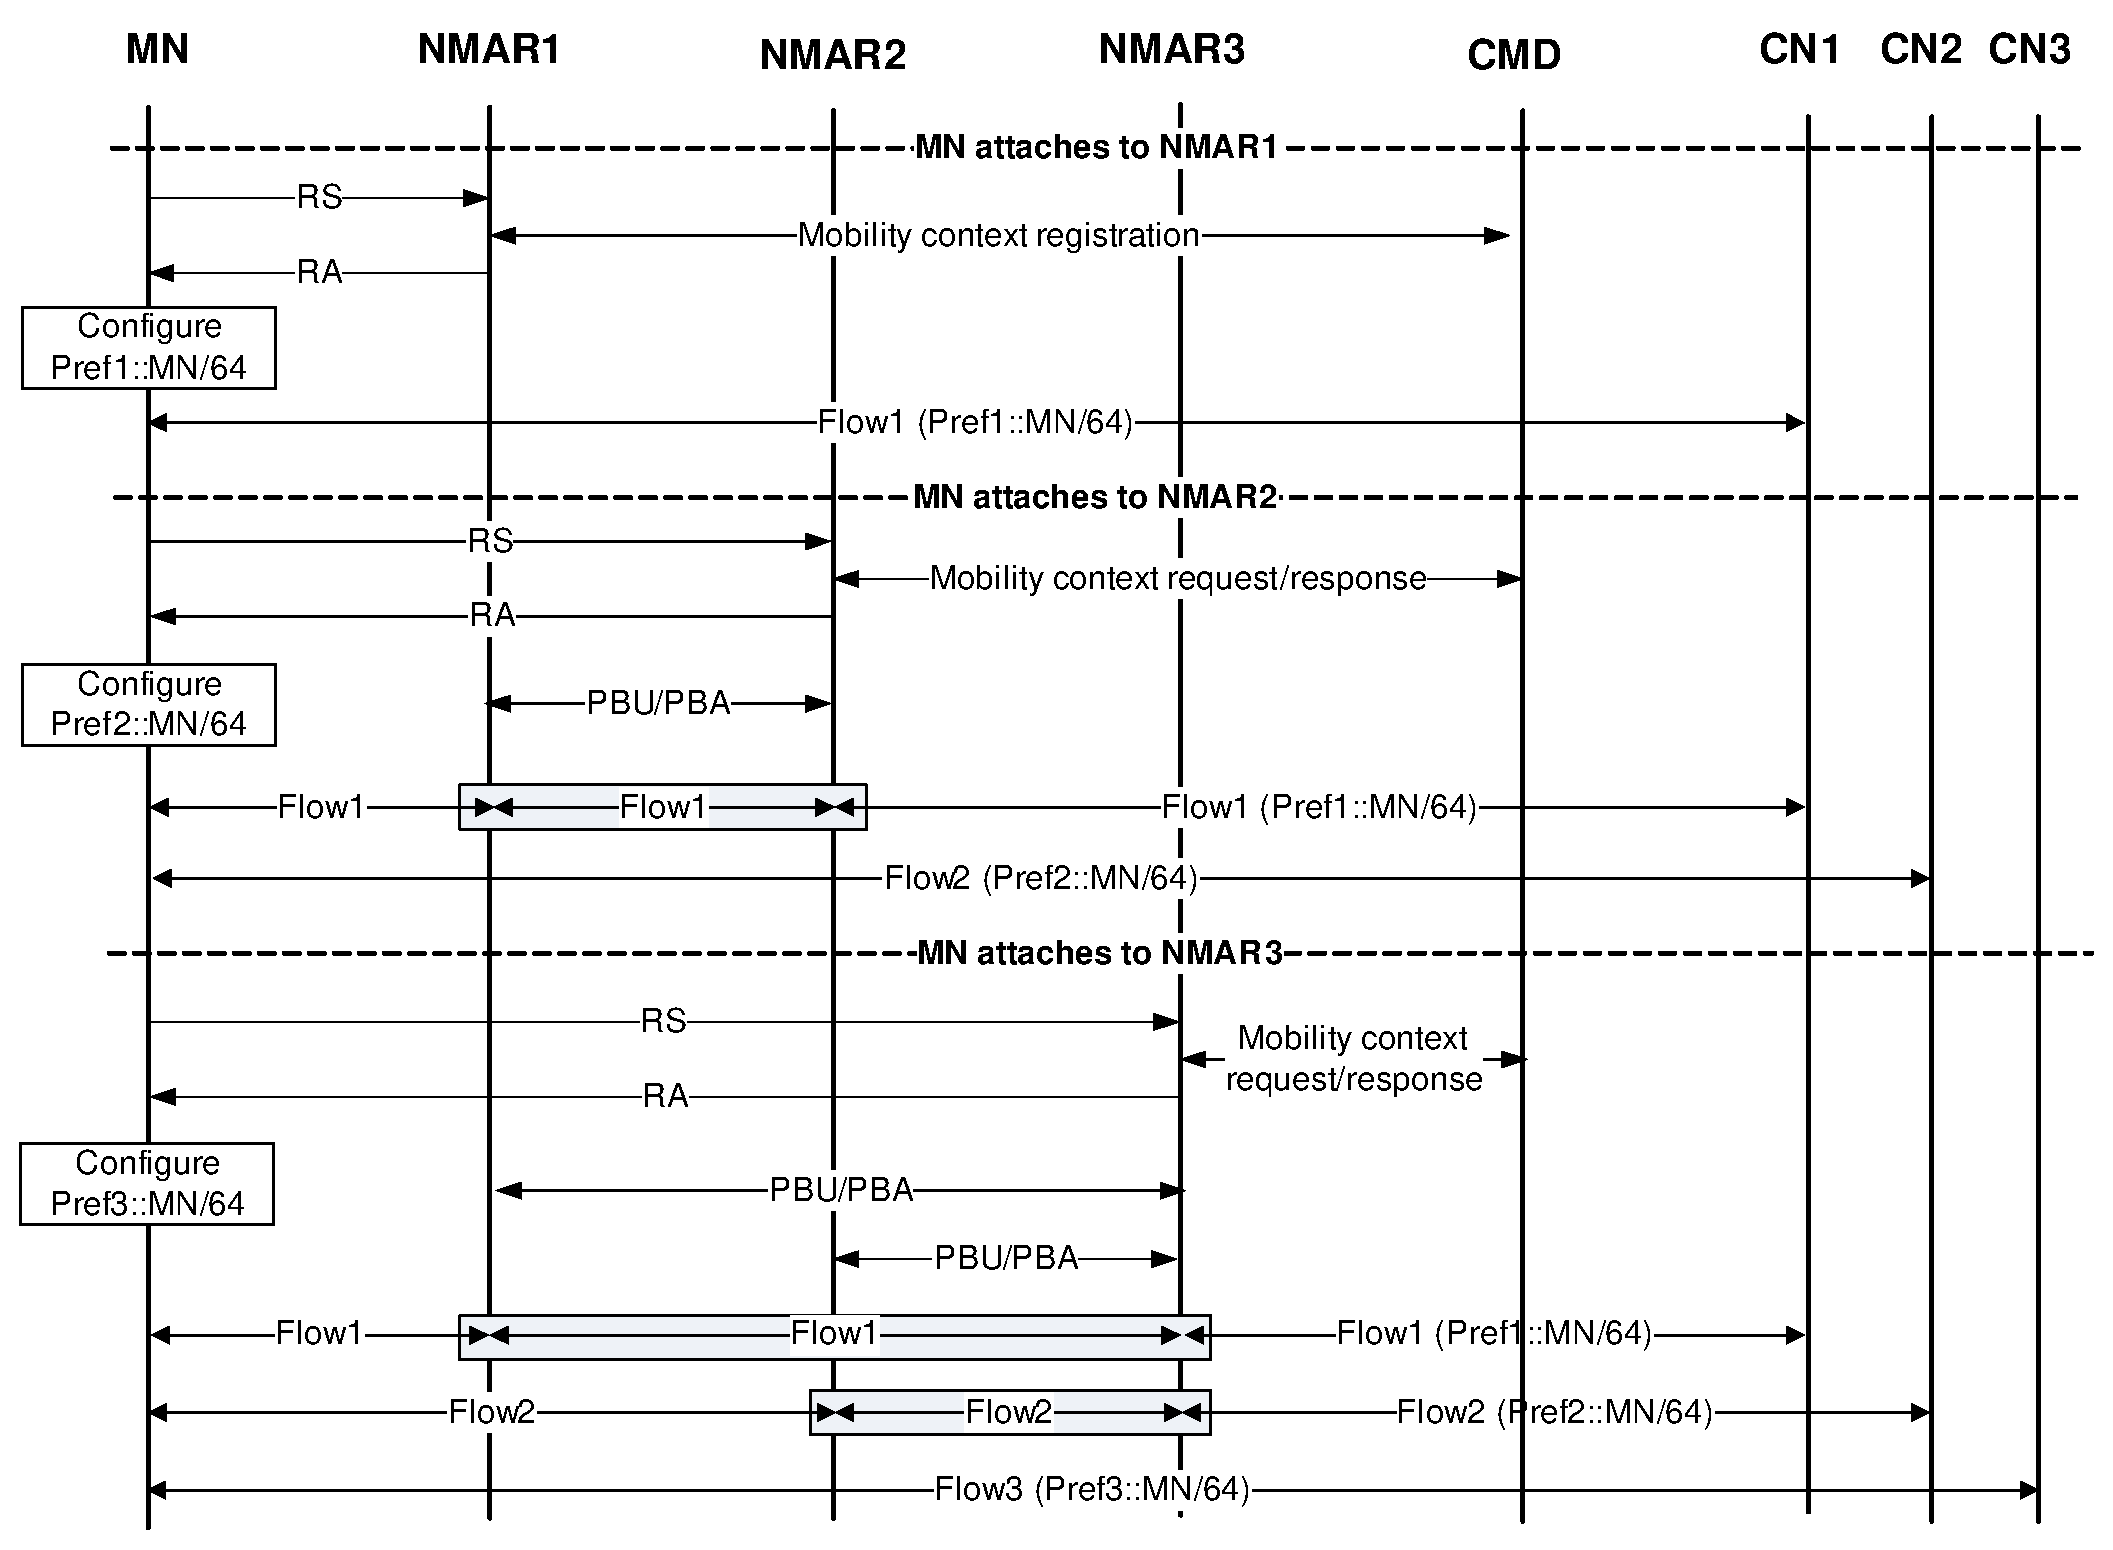
\includegraphics[width=0.9\textwidth]{./Part1/Chapter2/figures/c3_pmip_dmm_signaling.eps} 
    \caption{Signaling for the mobility management in the network-based approach.}
     \label{fig:c3_pmip_dmm_signaling}
  \end{center} 
\end{figure}

 The diagram in Fig.~\ref{fig:c3_pmip_dmm_signaling} depicts the operations of the partially distributed DMM. When an MN attaches to the network-based DMM domain (for example at NMAR1), after detecting the presence of a new MN by means of receiving a RS message (including the MN's ID), the NMAR1 allocates a HNP (Pref1::/64) for the MN. It then sends a mobility context request (MC-Req) message including the MN\_ID and the Pref1::/64 to the CMD to register the new prefix and retrieve the existing mobility context of the MN (if exist). The CMD then checks its mobility database for this MN. Since it is the first time the MN is attached to this domain, there is no entry for it. Therefore, the CMD creates an entry (for the MN) including the MN\_ID, Pref1::/64 and the associated NMAR (NMAR1). The CMD sends a mobility context response (MC-Res) message indicating that the information of the MN is successfully registered. Afterwards, the NMAR1 sends a RA including the allocated prefix (Pref1::/64) to the MN. Based on this information, the MN configures its IPv6 address (Pref1::MN/64) and starts a new communication with the CN1 (Flow1), following the normal way. As the MN moves to the access network of NMAR2,  the NMAR2 allocates a new HNP (let say Pref2::/64) for the MN. It then sends a MC-Req message to the CMD for the new prefix registration and for retrieving the existing mobility context of the MN. Upon receiving the MC-Req message and searching its mobility context table, the CMD updates the MN's mobility entry corresponding to the new prefix (as in Fig.~\ref{fig:c3_pmip_dmm}). The CMD then replies by a MC-Res message including the MN\_ID and the list of its active prefixes, and the associated NMARs (in this case is Pref1::/64 and NMAR1). Upon the reception of the MC-Res message, the NMAR2 updates its BCE and routing for Pref2 and sends a RA to the MN which includes the Pref2::/64. The PBU/PBA messages are then exchanged between the NMAR2 and the NMAR1 to sets up the bi-directional tunnel between them for the Flow1. Regarding the MN, after receiving a RA, it configures its IP address (Pref2::MN) and uses it to start a new communication with the CN2 (Flow2) in a normal way. The similar thing happens when the MN moves to NMAR3. In this case, the Flow1 and Flow2 are routed through the NMAR1 and NMAR2, respectively. In the mean time, the Flow3 which is initiated when the MN attaches to NMAR3, is routed in a normal way without the tunneling mechanism. 

Besides, there are proposals which apply the DMM concepts into the PMIPv6 domain. For example, in \cite{PMIP_based_DMM_Korhonen}, the locally assigned prefixes mechanism within a PMIPv6 domain is proposed. In this case, the MAG can attribute its own prefix (the so-called local prefix) to the MN which can be used for the communication by passing the LMA when the MN is currently attached to the MAG. The MN can still use the IP address allocated by the LMA in a typical PMIPv6 way.  
\subsubsection{DMM Consideration in 3GPP}
\begin{figure}[h!]
\centering
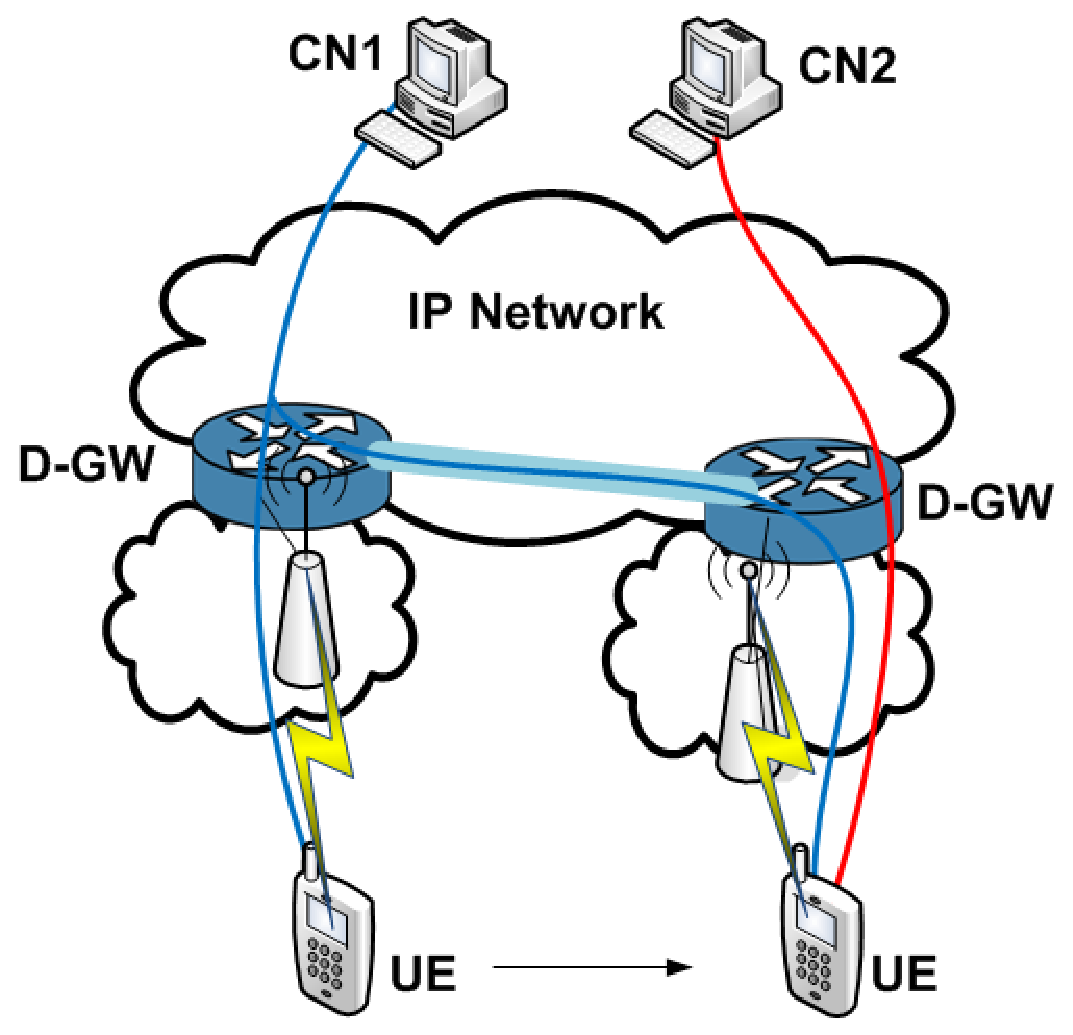
\includegraphics[width=0.38\textwidth]{./Part1/Chapter2/figures/c3_dmm_3gpp.eps}
\caption[Mobility management for 3GPP.]{Mobility management for 3GPP}
\label{fig:c3_dmm_3gpp}
\end{figure}

In order to deal with a huge number of traffic demands as well as the revenue per data decreasing phenomenon, 3GPP proposes such traffic offload mechanisms as SIPTO, LIPA and IP Flow Mobility (IFOM). The main idea is that the user data can be routed bypassing the core network based on certain conditions. In more details, SIPTO supports offload of certain types of traffic directly to the Internet and away from the mobile core network. It is done by selecting a set of S-GWs and P-GWs that are geographically/topologically close to the User Equipment's point of attachment (UE is an MN following the 3GPP terminology). However, the offloaded traffic cannot access the operator services. On the other hand, LIPA enables a UE connected via a Home eNB (HeNB) to access the IP capable entities in the same residential/enterprise IP network without the data traversing the mobile operator’s core. Although, SIPTO/LIPA is similar to DMM in terms of traffic offloading (mitigating the traffic aggregation at the core network), there is a limited mobility support. For example, LIPA supports only the mobility between HeNBs managed by the same Local-GW (L-GW) while SIPTO enables mobility support for the case S-GW/P-GW is at/above Radio Access Network (RAN). In other words, 3GPP has not yet considered the mobility of UE, which may result in service disruption when a UE is on the move. In fact, SIPTO/LIPA can be considered as a step towards DMM from conventional centralized/hierarchical approaches. It comes from the fact that based on SIPTO/LIPA the functionality of P-GW is distributed by deploying multiple L-GWs. In the next step, by re-using the existing S5 interface (PMIPv6 tunneling), the mobility between the L-GWs can be enabled. From that point, it is feasible to support DMM in LTE/SAE by simply installing the DMM functionality at the distributed L-GWs (called Distributed Gateway or D-GW) as illustrated in Fig.~\ref{fig:c3_dmm_3gpp}. 

\subsection{Other Considerations}
\subsubsection{Mobility across Heterogeneous Networks}
With the evolution of mobile communication systems (wireless technology and network architecture), heterogeneous networks provide the possibility to greatly increasing capacity at a low cost. In this context, the seamless mobility across different types of wireless access technology e.g., WLAN, WiMAX and LTE needs to be taken into account. Regarding the network infrastructure, IEEE 802.21 Media Independent Handover (MIH) services allow optimizing the handovers between heterogeneous IEEE 802 and cellular networks. The handover performance can be enhanced using the layer-2 information available from IEEE 802.21 services. From the mobile node point of view, to maintain the session continuity, additional techniques (as specified in \cite{PMIP_EV}) should be considered which allow the MN to obtain the same IPv6 address after handover across different access technologies. Among them, the logical interface technique \cite{logical_interface} can help to hide the different access technologies, thus, the changing of interface is transparent to the IP stack. Moreover, the interfaces of the MN can be active at the same time, which helps reducing the handover latency. 

\subsubsection{Network Mobility}
Network Mobility (NEMO)\footnote{NEMO IETF WG: http://datatracker.ietf.org/wg/nemo/} refers to the mobility of an entire network which changes its point of attachment to the Internet. Thus, the main purpose of NEMO support is that it allows every node in the mobile network to be reachable while moving around. Moreover, the mobility should be transparent to the nodes insides the mobile network. The basic network mobility support is based on MIPv6 to enable the network mobility in an IPv6 network. 

In order to provide the mobility support for a Mobile Network, a specific gateway called Mobile Router (MOR) is introduced. The MOR will be connected to the fixed infrastructure and provides connectivity to the nodes inside the Mobile Network. Like the mobility support of a mobile node (host-based approach), the NEMO basic support (as specified in \cite{NEMO}) is also based on the bi-directional tunnel between the MOR and its HA to enable mobility support when the MOR is away from home. Thus, as a topological anchor point of MOR's address, the data packets addressed to the mobile network are delivered to the HA, which then tunnel them towards the MOR. The MOR, after removing the tunnel headers, forwards the data packets to the destination inside the mobile network. Note that similar to normal MIPv6 operation where the binding association between the HoA and the CoA is maintained in the Binding Cache, in NEMO, the HA might also keep the Mobile Network Prefixes (MNP) in the corresponding BCE. As a result, in a large-scale development, the MNP allocation should be considered as in \cite{NEMO_DHCP}. 
 
\subsubsection{Comparison between the Mobility Management Approaches}
As stated earlier, the performance of a mobility management protocol is typically measured using such metrics as signaling cost, handover latency, and packet loss. Based on these metrics, various papers have been presented to evaluate the performance of the mobility management protocols. 

Comparative performance analysis for the host-based mobility management protocols e.g., MIPv6, FMIPv6, HMIPv6 and F-HMIPv6 in terms of signaling cost, handover latency, and packet loss has been carried out in \cite{HO_comparison_Montavont, HO_comparison_Makaya,HO_comparison_Costa}. In \cite{HO_comparison_Lee,HO_comparison_Lee_2,HO_comparison_Lee_3}, the authors also took into account the network-based mobility management protocols e.g., PMIPv6 and FPMIPv6 in the comparative performance analysis. From these analysis, some conclusions are: i) Using layer 2 information generally helps to reduce the handover latency and packet loss at a cost of signaling overhead. However, it depends on each link-layer technology; ii) The network-based mobility management protocols reduce the signaling overhead over the air of the MN compared to the host-based mobility protocols; and iii) Typically, the handover latency and the signaling cost depend on the network topology in use. In other words, the hop distance between the network entities is an important factor influencing the performance of these protocols.  

Regarding DMM, a lot of research publications \cite{DMM_Bertin, PMIP_based_DMM_Giust, DMM_IETF_Lee, MIP_based_DMM_Condeixa, MIP_based_DMM_Hassan, DMM_analysis_Hassan} have carried out the analysis on different DMM approaches, compared them with the conventional mobility managements in terms of signaling cost, packet delivery cost, handover delay, packet loss and end-to-end delay. The results from these analysis showed that DMM is a promising mobility management scheme. In details, in \cite{DMM_Bertin} the authors conducted a simulation to compare DMM and MIPv6 (with handover optimizations). The simulation results showed that DMM outperforms MIPv6 in terms of handover delay and TCP delay. In \cite{DMM_IETF_Lee}, both qualitative and quantitative comparison for centralized mobility management protocols and DMM protocols are provided. Also, the comparison in terms of handover latency, signaling cost and data delivery cost has been conducted in \cite{MIP_based_DMM_Condeixa}. 

\section{IP Mobile Multicast}
The increasing penetration of the mobile devices, such as tablets and smart phones is generating a huge number of data traffic over mobile networks. The majority of this traffic is video data: estimates say that mobile video traffic will account for 66.5\% of total mobile data traffic by 2017 \cite{cisco_forecast}. In this context, the scalability and the bandwidth efficiency from the multicast routing make the IP multicast a remarkable solution from application point of view to allow mobile networks to deal with a huge number of traffic, particularly in mobile environments where users usually share frequency bands and limited capacity \cite{Multicast_MIPv6}. In other words, when a large group of users is simultaneously interested in the same content, the multicast can provide significant advantages compared to the unicast in terms of resources efficiency both from the perspectives of the network and of the servers \cite{developing_ip_multicast}. However, one of the major challenges for multicast support is when mobility is considered.

About the IP mobile multicast, after more than a decade of research and development efforts, many approaches have been proposed, but most of them are based on such host-based mobility management protocols as MIPv6, FMIPv6 and HMIPv6. However, the main drawback of these host-based mobility management protocols is that they require the MN to modify its IP stack to participate into the mobility signaling process. As a result, the previous IP multicast approaches introduced in \cite{Multicast_MIPv6, multicast_challenges_solutions} cannot be directly applied in a network-based mobility management in which the MN is unaware of the mobility process.

Recently, a base development of multicast listener support in PMIPv6 has been adopted by the IETF. However, it does not provide any specific optimization and performance enhancements such as service disruption and packet loss, sub-optimal routing, and packet duplication. Several solutions have been proposed in order to address couple of issues. In this section, we give a brief overview to the multicast mobility-related problems and enlist some possible solutions in MIPv6 to highlight the main idea of these proposals. Based on that, we then take a deep analysis on the multicast mobility in a PMIPv6 and a DMM environment. 

\subsection{Overview of Multicast Mobility in Mobile IP}
In order to enable multicast in Mobile IP (both Mobile IPv4 and Mobile IPv6), two basic approaches have been proposed i.e., bidirectional tunneling and remote subscription. Both approaches have their own advantages and drawbacks. The bidirectional tunneling hides the movement of the multicast nodes by tunneling the multicast traffic via the mobility tunnel between the node and its HA at the cost of triangular routing (leading to a long delay) and tunnel convergence problem. On the other hand, in the remote subscription approach, the multicast node has to rejoin the on-going multicast sessions after each handover, leading to the potential significant service disruption. In addition, more serious problems can be raised in case of source mobility such as address transparency and routing state maintenance \cite{Multicast_MIPv6, multicast_challenges_solutions}. Further enhancement should also be considered in order to meet the additional requirements in terms of service disruption and packet loss for the real-time services. Therefore, various methods have been proposed to improve the two essential solutions. In \cite{multicast_challenges_solutions,Multicast_MIPv6}, the authors provides a survey of numerous proposals for the multicast listener as well as the source mobility. 

From listener point of view, several solutions \cite{MoM, RBMoM,MPDSR, MMA} have been proposed to construct an efficient multicast delivery tree. In more details, the Mobile Multicast Protocol (MoM) \cite{MoM} aims at solving the tunnel convergence problem by selecting one HA which serves as a common HA (per group) for all listeners subscribed to a multicast group at the same visited network. In other words, a single tunnel between the selected HA and the FA is used for multicast delivery between the home network and the foreign network. The Range-Based Mobile Multicast (RBMoM) \cite{RBMoM} trades off the shortest delivery path and the frequency of multicast delivery reconstruction, however, it introduces much of complexity. The Multicast Protocol With Dynamic Service Range (MPDSR) \cite{MPDSR} enhances RBMoM to reduce the number of multicast tree reconstructions and multicast service disruption time. In general, MoM, RBMoM and MPDSR can be considered as an enhancement of the bidirectional tunneling approach. The Multicast By Multicast Agent Protocol (MMAP) \cite{MMA}, as an enhancement of the remote subscription approach, uses the tunnel between the previous foreign network and the current one for delivering the multicast traffic to reduce the tunnel convergence problem and the service disruption. In \cite{multicast_ip_Jelger}, the authors proposes combining the bidirectional tunneling and the remote subscription. They also discusses the practical aspects of the bidirectional tunneling approach. Besides, \cite{seamless_multicast_MIPv6, FPMIPv6_multicast,fast_multicast_Kwon} mainly aim at addressing the problem of packet loss and multicast service disruption by extending the fast handover protocols for multicast support.  

From multicast source point of view, the bidirectional tunneling approach preserves the transparency of the movement of the source. However, it suffers the triangular routing, long service latency, and inefficient in packet delivery which impact the overall listeners. The remote subscription approach helps to address these issues, yet, the movement of the source causes the address transparency and tree reconstruction. Thus, the multicast routes should be updated to reflect the current location of the source in an appropriate manner to effectively avoid the packet loss. There are two main types of solution in which the traffic will be injected to the old tree or the overall delivery tree will be reconstructed \cite{Multicast_MIPv6}. The additional complexity is raised in case of SSM. For example, in \cite{tree_morphing_Schmidt, tree_morphing_Christ}, the authors propose a tree morphing protocol to address the address transparent issue allowing a continuous adaptation of multicast shortest path trees to the source mobility. However, the complexity and high signaling cost could be added, as all the MRs need to be extended. Similarly, in \cite{PMIP_multicast_source_Lee}, the authors propose a state update mechanism by reusing the legacy multicast tree for a minimization of packet delay. In \cite{host_identity_multicast}, the authors, based on the Host Identity Protocol, introduce multicast routing states which is independent of IP addresses. Further approaches can be found in \cite{multicast_challenges_solutions,Multicast_MIPv6,multicast_source_Wang}. 

Since all these mobile multicast protocols are designed for MIPv4 and MIPv6 which require the mobile nodes to participate in the signaling process, they cannot be directly applied to PMIPv6. Yet, the idea of these solutions can be re-used. 

\subsection{Multicast Mobility in PMIPv6}
As the multicast protocols (group management and routing protocols) are originally designed for a fixed network, considering multicast in a mobile environment brings several challenges to the multicast service. The mobility of the node  (e.g., the change of point of attachment and of globally reachable IP address) has different impacts on the multicast service, depending on such factors as the role of the node in the multicast session (source or listener), the considered multicast model (ASM or SSM), the multicast routing protocol, the multicast group management protocol and the mobility protocol in use as well as the wireless access technology. Therefore, the IP mobile multicast issues can be divided into four main groups: the general multicast problems (due to multicast protocols), the specific mobile listener problems, the specific mobile source problems and the deployment issues \cite{Multicast_MIPv6, multicast_challenges_solutions,tuning_MLD}.

\subsubsection{Multicast Mobility Issues}
Prior to taking more details on the multicast mobility issues, we will look at some requirements of the multicast support in PMIPv6. First, the session continuity should be provided when a listener/source moves from one IPv6 subnet to another. In addition, the noticeable service disruption and the significant packet loss should be avoided during handovers. Especially, in the context of a network-based mobility management protocol, the mobile node should remain unaware of mobility from the network layer and the application point of view. Then, it is desirable to preserve the characteristics of multicast such as effectiveness of delivery (to avoid traffic duplication and tunneling overhead) and approximate optimal routing. 

\paragraph{General Issues}
At the beginning, the multicast protocols are designed for a fixed environment using wired connection. Thus, considering these protocols in a mobile and wireless environment can raise several challenges. Particularly, considering the multicast group management protocols (IGMPv3 and MLDv2), which typically work in the wireless access network (MN and first hop AR), may lead to such issues as the multicast-related signaling overhead, the multicast service disruption and the long leaving latency \cite{tuning_MLD}. Additionally, wireless is typically an unreliable media, that means variable bandwidth or packet losses, and overall wireless communications are more costly (both in power and processing overhead). As such, the tuning of MLDv2 parameters (timers and values) \cite{tuning_MLD} must be considered for obtaining an improved multicast service stability and for a better behavior during handovers. Regarding multicast routing protocols, the movement of source and listener results in several issues such as tree reconstruction, routing state maintenance and tunneling, etc \cite{multicast_challenges_solutions}. Specifically, the tree reconstruction may lead to a long service disruption time and a significant packet loss. Adding to that, it is not easy to modify the multicast routing protocols according to mobility requirements. 

\paragraph{Specific Multicast Listener Mobility Issues}
The mobility of a listener causes several issues for the multicast service. The issues and the possible solutions are described as follows:
\begin{itemize}
\item  Service disruption and packet loss: Since the mobile node in the network-based mobility management is not aware of the mobility process, it cannot make multicast-related decisions, preventing a smooth multicast session resume. As a result, when a listener moves to a new MAG, it has to wait to express its interest in subscribing to the on-going multicast channels until it receives an MLD Query (from a Querier). Thus, it experiences a certain delay in receiving multicast content due to the extra time related to the multicast service activation, the MLD Query/Report transmission (especially the multicast service activation which is typical in seconds). In other words, beside the layer 2 and layer 3 handover latency, the extra delay related to multicast service is added to the total latency. Also, if no buffer mechanism is used, the multicast traffic is discarded during handover, causing packet loss. This issue becomes more serious when the real-time services are considered, but can be reduced by using the context transfer function \cite{d4.2,d4.3,SIAL}.
\item Packet duplication: In some cases, the MAG can receive the same multicast packet from different LMAs or MRs. This happens when different tunnels MAG-LMA are used to deliver the multicast traffic. One possible solution is implementing MLD proxy with multiple upstream interfaces at MAG. Other possibility is taking advantage of the native multicast infrastructure to deliver multicast traffic, thus bypassing the tunnel \cite{direct_routing_mtma}.  
\item Sub-optimal routing and end-to-end delay: When the multicast traffic has to pass through the central mobility anchor (LMA), it often results in a longer route. Consequently, the end-to-end delay will be increased. This issue should be taken into account especially when the real-time and delay sensitive services are considered. 
\item Leave latency or network resource waste: Since the listener is unaware of mobility, it will not send an MLD report for explicitly leaving the group in the previous MAG (pMAG). As a result, if the last member of a multicast group moves to another MAG, the pMAG will continue to deliver the multicast traffic until it updates its membership information. Thus, it causes waste of network resource. Using the explicit tracking function \cite{explicit_tracking} and the context transfer, in this case, could help. 
\end{itemize}

In addition, the listener can receive the packet out of order due to handovers. In many wireless regimes, multicast-related signaling should be minimized to reduce the power consumption (of a limited capacity mobile devices) and network resource (with a limited capacity) in use. Again, tuning the MLD parameters \cite{tuning_MLD} should be carefully investigated as a trade-off of signaling overhead and service disruption as well as waste of resources issue. 
  
\paragraph{Specific Multicast Source Mobility Issues}
From a source point of view, it inherits some problems of the multicast listener mobility such as service disruption, packet loss and sub-optimal routing. Particularly, since the movement of a multicast source between different networks could impact overall multicast delivery tree, it may cause more severe problem in terms of service disruption and packet loss if multicast tree needs to be reconstructed. As in PMIPv6, the source keeps its IPv6 address when moving across a PMIPv6 domain, the address transparency issue is avoided. However, if the multicast traffic is routed directly from the MAG bypassing the LMA, it may lead to several issues such as packet overhead, encapsulation/decapsulation cost, source register tunnel management and sub-optimal routing \cite{PIM_SM, multicast_source}. Additional issue may be raised from the multicast scoping and source active when considering inter-domain mobility. The impact of source mobility, in general, strongly depends on the multicast deployment scenario as well as the multicast model considered (ASM or SSM). In SSM, the traffic follows the shortest path tree rooted at the source to the listeners. As in PMIPv6, LMA always acts as a topological anchor of the source's address, the traffic has to pass the LMA after forwarding to the listeners. It leads to the non-optimal route. As a result, additional mechanisms are required to enable the optimal route in case of SSM. However, the simplicity feature, as a main advantage of SSM, should be taken into account. In ASM, the presence of the RP can help to hide the mobility of the source since the source address is preserved when it attaches to the PMIPv6 domain. However, when the listener's DR decides to switch to the shortest-path tree, the similar issues as in SSM should be considered. 
\paragraph{Deployment Issues}
After more than a decade of important research and development efforts, IP multicast, in general, has been slowly deployed on the global Internet (lagging but still growing). The barrier of widespread deployment of multicast applications mainly comes from technical, administrative and business related issues as stated in \cite{alternative_multicast}. Therefore, several alternative techniques for multicasting have been proposed \cite{alternative_multicast}, in which each alternative can be suitable for a specific environment. For example, the application-layer multicast (ALM) \cite{application_multicast} in which the multicasting functionality is implemented at the application layer instead of at the network layer as IP multicast, does not require the change in the network infrastructure. Data packets are replicated at the end hosts, instead of the network routers as in IP multicast. ALM is suitable, for example, for the MANET applications. Although ALM is much easier to deploy compared to IP multicast, IP multicast over performance the ALM (as well as other alternatives) in terms of robustness, security, performance, and scalability \cite{alternative_multicast}. The recent business models, a huge traffic demand (especially multimedia traffic), the revenue per data reducing phenomenon in the mobile operator networks, as well as the advantages of new multicast model (SSM) bring again the strong interest of IP multicast from both academic and industry communities. IP multicast is expected to play more important role in the future networks. 

\subsubsection{Solutions from the IETF Point of View}
Following a typical multicast deployment architecture, multicast support can be enabled by deployed an MLD proxy and an MR function in the domain. In general, different proposals for multicast mobility in PMIPv6 are derived from the mapping the location of MAG and LMA into the typical multicast deployment architecture, as shown in Fig.~\ref{fig:c4_mapping_pmip}. As a result, there are three approaches corresponding to the different roles of MAG and LMA as: i) MAG and LMA act as an MLD proxy and an MR, respectively; ii) MAG acts as an MLD proxy while LMA as an additional MLD proxy; and iii) MAG and LMA play the role of an MR. 

The first approach, which is considered as a base solution by the IETF, enables the multicast support by deploying MLD proxy and the multicast routing function at MAG and LMA, respectively. This solution can also be considered as a tunnel-based solution due to the fact that the multicast traffic is routed via the mobility tunnel between LMA and MAG. In addition, LMA can also act as an additional MLD proxy (in the second approach). In the third approach, by deploying multicast routing at MAG, several issues can be avoided (e.g., sub-optimal routing, tunnel convergence problem) at a cost of operation and deployment from the multicast routing.
\begin{figure}[h!]
\centering
\includegraphics[width=0.80\textwidth]{./Part1/Chapter2/figures/c4_multicast_mapping.eps}
\caption[Mapping PMIP entities into the multicast deployment architecture]{Mapping PMIP entities into the multicast architecture}
\label{fig:c4_mapping_pmip}
\end{figure}

At the time PMIPv6 protocol was developed, it does not explicitly address the multicast communication. Consequently, a new IETF group, namely MultiMob\footnote{MultiMob WG: http://datatracker.ietf.org/wg/multimob/charter/}, has been chartered for supporting multicast in a mobile environment. At this stage, the PMIPv6 multicast listener support was standardized while the multicast sender support is still under discussion. 

\paragraph{Solutions for Multicast Listener Mobility\\ \\ }
This subsection presents different possible solutions for multicast listener mobility in PMIPv6 mainly from the IETF point of view. Starting with a base solution which does not take any performance and optimization issues into account, we then consider the solutions for some specific issues as stated in the previous subsection. 

\subparagraph{Base Solution for Multicast Listener Mobility in PMIPv6}
Recently, a base solution \cite{RFC_6224} has been standardized by the IETF for supporting multicast listener mobility in PMIPv6 without modifying the mobility and multicast protocol standards. It provides multicast listener support in PMIPv6 by placing MLD proxy function at MAG while LMA acting as an MR or an additional MLD proxy (see Fig.~\ref{fig:c4_mapping_pmip}). The MLD proxy function is implemented at MAGs with the upstream interface being configured to the corresponding mobile node’s LMA (ingress interface). As a typical MLD proxy operation, the multicast data arriving from an upstream interface will be forwarded to the downstream interfaces which have appropriate forwarding states for this group. Thus, all multicast traffic will pass through the MAG-LMA tunnel, just like the unicast traffic. This solution can be considered as a tunnel-based one. After each handover, the multicast traffic continues to deliver to the listener at the new MAG, and the service continuity is guaranteed accordingly. In addition, from the multicast service point of view, the listener remains unaware of the mobility. It is achieved since the new MAG, after obtaining the listener's subscription information by using the normal MLD operations, joins the on-going multicast flows on behalf of the listener. The base solution can be also applied for the multicast source \cite{multicast_source}. Note that the LMA can also work as an additional MLD proxy, serving multicast traffic for the PMIPv6 domain. However, from the listener and the MAG perspective, there is no difference. Therefore, without loss of generality, we only consider the case where the LMA acts as an MR.
\begin{figure}[h!] 
 \begin{center} 
 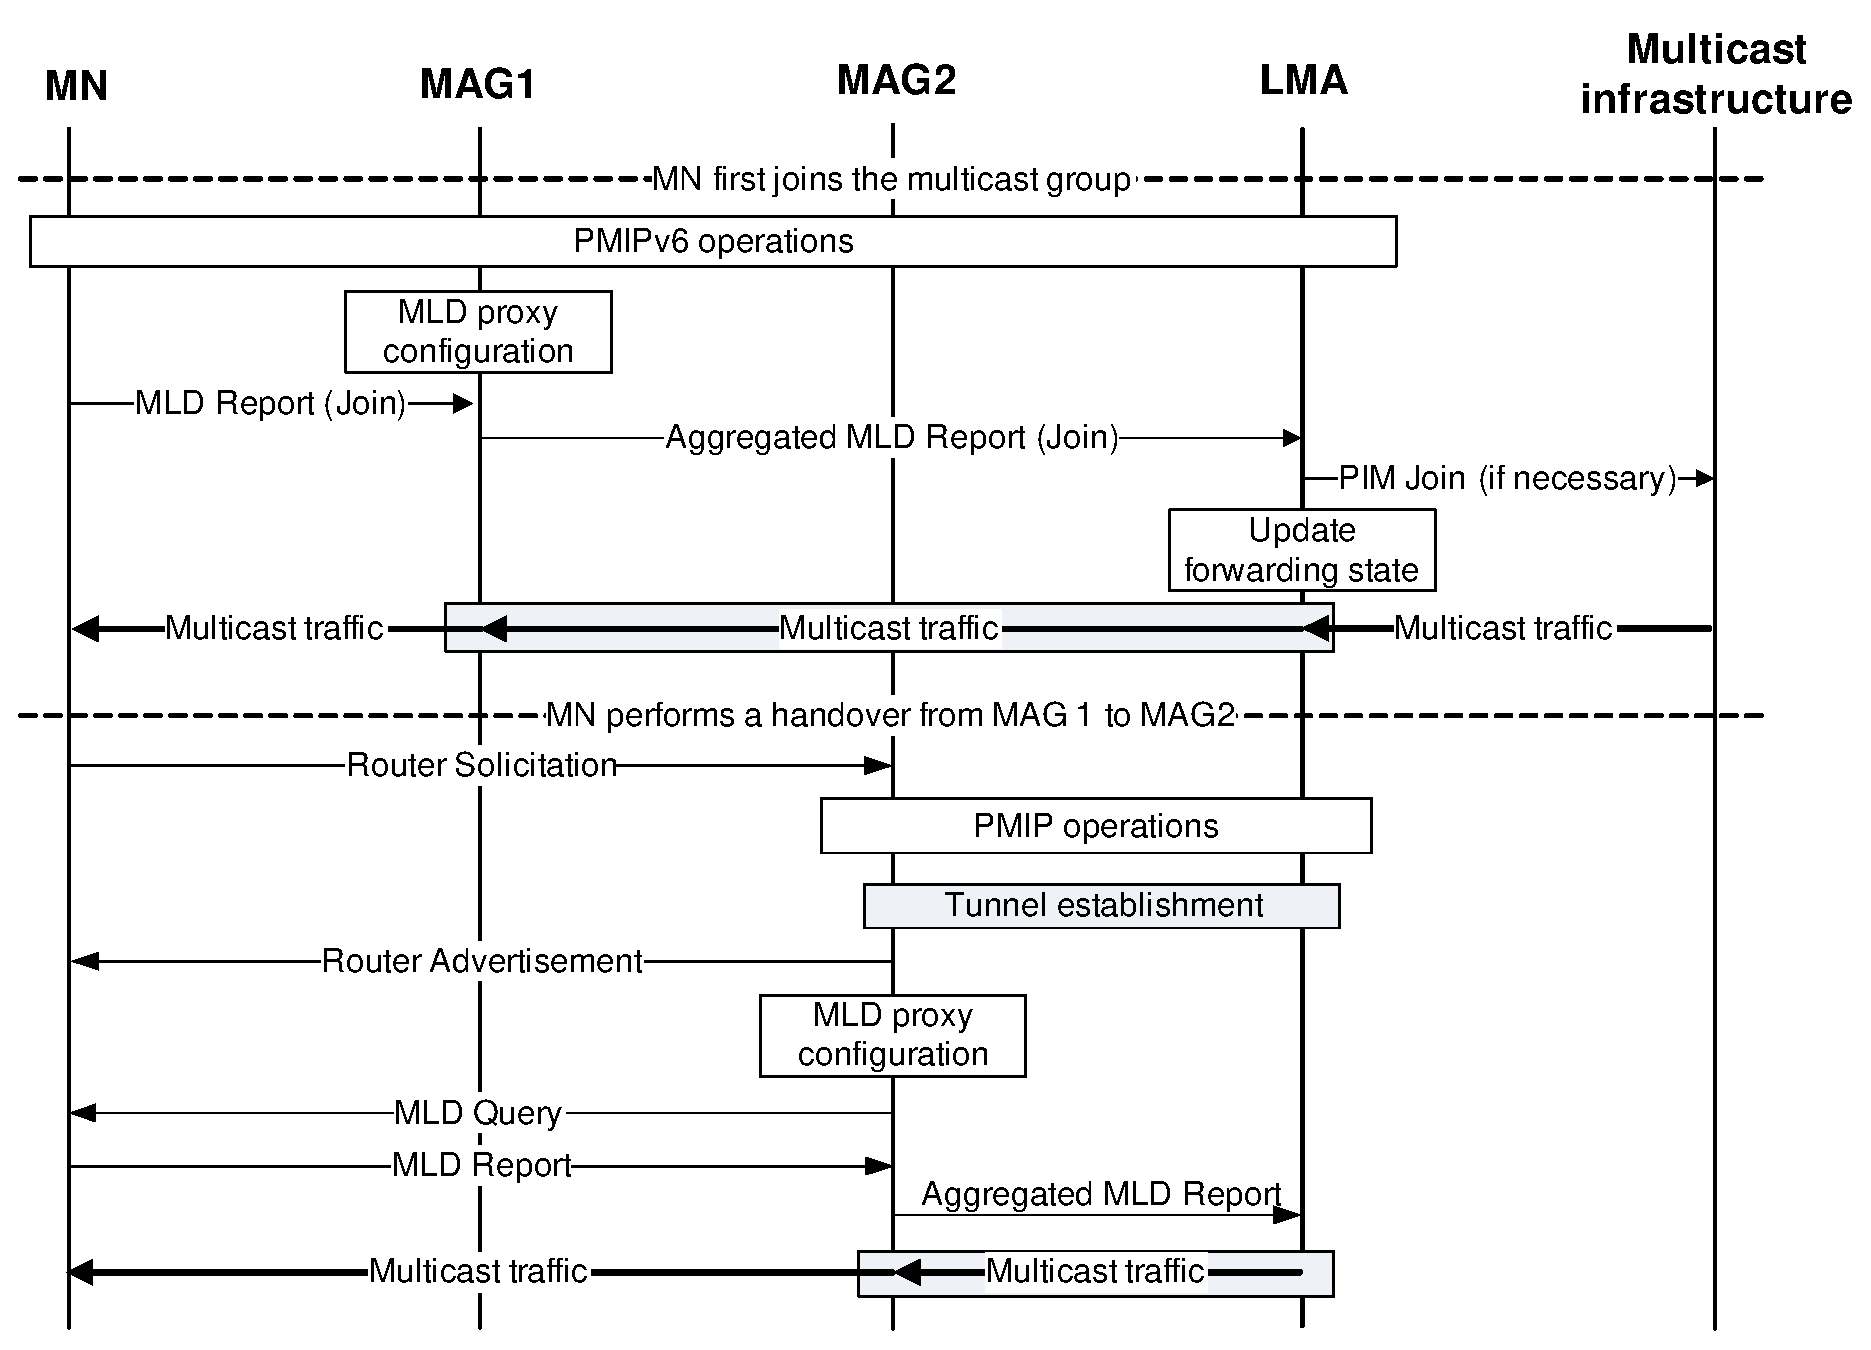
\includegraphics[width=0.85\textwidth]{./Part1/Chapter2/figures/c4_base_solution.eps} 
    \caption{Base solution for multicast listener mobility in PMIPv6.}
     \label{fig:c4_base_solution}
  \end{center} 
\end{figure} 

Fig.~\ref{fig:c4_base_solution} describes the multicast-related signaling for the base solution. When an MN is initially attached to a PMIPv6 domain (for example, attaches to MAG1), first, the standard PIMPv6 operation will be executed (e.g., MN's address configuration, MN's location update, tunnel establishment, for more details see Section \ref{c1:IP_Mobility}). MAG1 then creates an MLD proxy instance (if necessary) which serves as an upstream router for all the nodes associated with the MN's LMA. Note that every MAG-LMA tunnel is a part of a separate MLD proxy domain. The proxy instance adds the MN to its downstream interface and configures its upstream interface towards the MN's LMA. When the MN expresses its willingness in receiving the multicast traffic from a group, it sends an MLD Report to MAG1. MAG1 then sends an aggregated MLD Report message to the LMA to join the group on behalf of the MN. The LMA, acting as an MR, joins the group from the multicast infrastructure, and updates its multicast forwarding state. After receiving the multicast packets, the LMA forwards them to the appropriate MAGs according to its forwarding state (via the LMA-MAG tunnel). MAG1 forwards the packets to the appropriate downstream interfaces and they finally reach the MN. \\

In case of handover (from MAG1 to MAG2), the basic PIMPv6 operation will be executed. Since the mobility is transparent to the MN, the MN will not send the unsolicited MLD Reports. Instead, MAG2, upon the detection of a new MN on its access link, adds the MN to a downstream interface, and sends MLD General Query messages on its attached link. The MN then replies by an MLD Current State Report message indicating its current active multicast groups. Based on that, MAG2 can send an aggregated MLD Report message to the corresponding LMA to join the groups on behalf of the MN (in case MAG2 is not receiving such those multicast groups). After updating the multicast forwarding state, the LMA forwards the multicast packets to the appropriate MAGs (including MAG2). The multicast packets finally reach the MN. 

Although the base solution is a simple way to enable the multicast support in PMIPv6, it does not address any issues as specified in the previous section. In more details, the utilization of tunnel for multicast flow results in the traffic redundancy (or the tunnel convergence problem) at the MAG. It is because different nodes, which attach to the MAG and associate to different LMAs, can subscribe to the same multicast group. There are several solutions for this issue such as extending MLD proxy to support multiple upstream interfaces \cite{multi_upstream_interface}, or using the direct-routing approach \cite{direct_routing_mtma}. Also, since a lot of operations need to be executed to allow the MN to continue receiving the multicast traffic at the new MAG, it may cause a long service disruption and high number of lost packets. This issue can be mitigated by either using the context transfer from previous MAG/LMA to the new MAG \cite{d4.2,SIAL} or tuning the behavior of MLD for routers \cite{tuning_MLD}. In addition, as the multicast traffic always passes through the MN's LMA, it may cause the sub-optimal routing problem. Possible solutions for this problem can be a localized multicast traffic and using a direct routing. 

\subparagraph{Direct-routing Solution} 
In order to provide an optimal connectivity to a local content, the direct routing approach which uses native multicast infrastructure locally in a PMIPv6 domain is proposed \cite{direct_routing_mtma}. In this case, the MLD proxy is implemented at MAG in which the upstream interface is configured towards an MR in the multicast infrastructure. Therefore, the direct routing approach helps avoid the tunnel convergence problem. One of the most important advantages of this approach is that multicasting functions are totally separated from the mobility anchor by using the native multicast infrastructure. As the result, the complexity of LMA is reduced since it does not have to deal with the multicast traffic processing. In addition, this approach may not make any packet overhead (tunneling overhead) as the multicast traffic is not transferred via the mobility tunnel. However, if the tunneling mechanism is used to set up the upstream interface of the MLD proxy towards an MR, the tunneling overhead can be re-introduced \cite{direct_routing_mtma}. 

The multicast-related operation in the direct-routing approach is briefly expressed as follows. Once an MN is attached to MAG1, similar to the tunnel-based approach, a proxy instance at MAG1 adds the MN to a downstream interface and configures its upstream interface towards an MR in the multicast infrastructure. Again, when the MN expresses its interest in receiving the traffic destined to a multicast group, MAG1 sends an aggregated MLD Report message to its upstream MR to join the group on behalf of the MN. Afterwards, the multicast traffic traverses the multicast infrastructure and reaches the MN. The MN then performs a handover to the new MAG, namely MAG2. Since the MN is unaware of the mobility process, it has to wait until receiving an MLD Query to inform its multicast information state to MAG2 by means of the MLD Current State Report message. MAG2 then joins the multicast delivery tree on behalf of the MN. MAG2 has to get the multicast traffic from an MR in the multicast infrastructure which already has a multicast forwarding state for this group. In other words, the multicast delivery tree needs to be reconstructed. Thus, it may result in a noticeable service disruption and packet loss. Some mechanisms are required to make sure that the multicast session continues right after the MN is attached to the new MAG and minimize the overhead in reconstructing the multicast trees. To tackle these issues, in \cite{direct_routing_mtma}, the authors propose to use a common upstream MR for all MAGs in the domain. Additionally, MAG can implement the MR functionality, in this case, MAG belongs to the multicast-enabled domain. 

In the same document \cite{direct_routing_mtma}, the authors propose separating the multicast from PMIPv6 unicast to solve the tunnel convergence problem. In more details, the multicast tree mobility anchor (MTMA), acting as an MLD proxy or an MR, is introduced to serve as a topological anchor point for the multicast traffic. In other words, while the multicast traffic is served by the MTMA, the unicast traffic is served by the typical LMAs. Typically, the MTMA would be used to get access to the remote multicast content, while direct routing to the local multicast content. In this case, PBA message should be extended to convey dynamic policies on subscription via MTMA/direct routing. 

\paragraph{Additional Considerations \\}
In case of handover, several operations should be executed so that the MN can continue receiving the multicast traffic from the nMAG: i) Typical PMIPv6 operations (e.g., exchanging PBU/PBA, tunnel establishment and address configuration); ii) Acquisition of the MN's multicast subscription information at the nMAG: Since the mobility is transparent to the MN, the service continuity is responsible by the nMAG through joining the ongoing multicast channels on behalf of the MN. To do so, the nMAG first needs to get the active multicast subscription information of the MN. It is done by relying on the normal MLD operations or the multicast context transfer mechanism; iii) Joining and getting the first multicast packet: The nMAG then decides joining the on-going multicast channels from its upstream MR/or an additional MLD proxy. Afterwards, the MAG forwards the multicast packets to the MN. 
From the multicast service point of view, while the information acquisition operation may lead to the service disruption and signaling overhead, the joining process depending on the position and the role of the upstream MR can cause the service disruption, signaling overhead, tunnel convergence problem and tunneling overhead. Regarding the service disruption time, it depends on all the operations. However, from the multicast service perspective, only the subscription acquisition time and joining time can be reduced for accelerating the multicast delivery. As a result, there are two possible solutions for these issues. The first one \cite{SIAL, FPMIPv6_multicast, tuning_MLD, Thinh_WCNC_Multicast} aims at reducing the time for information acquisition operation. The detailed discussions on this solution will be provided in Chapter \ref{ch:multicast_PMIP}. The second one mainly focuses on reducing the time needed for the joining process. Moreover, in both solutions, the operations during handover can be executed in parallel.   

\paragraph{Solutions for Multicast Source Mobility \\}
Limited work on the multicast source mobility in PMIPv6 has been developed compared to the multicast listener mobility. From the IETF point of view, the base solution for the multicast source mobility in PMIPv6 is still under discussion. In \cite{multicast_source}, the authors suggest using the base solution for listener for source mobility. In this case, MLD proxy and MR function need to be deployed at MAG and LMA, respectively. As a proxy, the packets arriving from a downstream interface will be forwarded to all the downstream interfaces which have the subscription information of this group except the incoming one and to the upstream interface. As a result, the multicast traffic from a local source will reach all the listeners attaching to the same MAG and sharing the same LMA (serving by the same MLD proxy instance). Serving as an upstream MR, the multicast traffic will be transmitted to the LMA, which then will be forwarded along the multicast delivery trees according to the forwarding state to reach all the listeners.

After a handover, the source can continue to send the multicast packets as soon as the MLD proxy at the nMAG maps the source to the corresponding proxy instance and the standard PMIPv6 operations are completed. The detailed operation is illustrated in Fig.~\ref{fig:c4_source_base}. It is worthy to note that when the source and listeners are attached to the same MAG but associated to different LMAs, the traffic will be routed in a definitely non-optimal route from the source's MAG to the source’s LMA, passing the listener’s LMA and finally returning to the same MAG. This is called a detour routing issue. 
\begin{figure}[h!] 
 \begin{center} 
 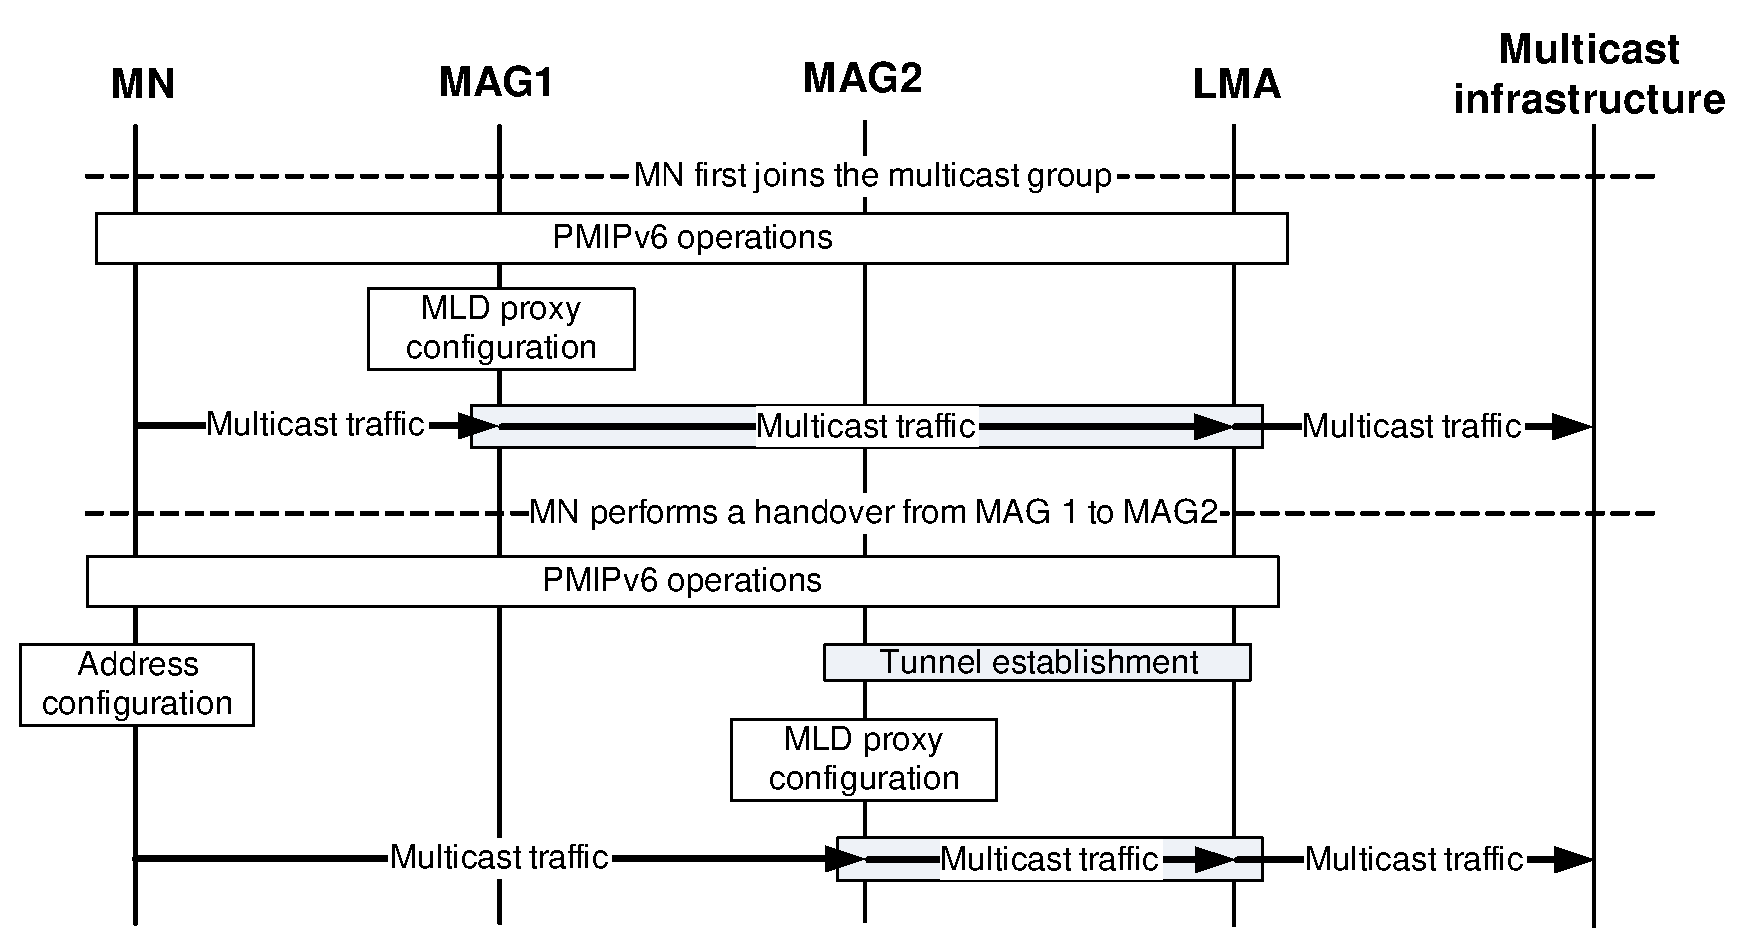
\includegraphics[width=0.75\textwidth]{./Part1/Chapter2/figures/c4_source_base.eps} 
    \caption{Signaling for the multicast source mobility support in PMIPv6.}
     \label{fig:c4_source_base}
  \end{center} 
\end{figure}

At the same document \cite{multicast_source}, the authors propose another possibility in which the multicast traffic is routed directly from MAGs to the multicast infrastructure bypassing the LMA (direct-routing). The direct routing can be supported by: i) MLD proxy deployment at MAGs with the upstream interface configured towards a common MR in the multicast infrastructure; or ii) the multicast routing protocol deployment at MAGs.  

In the former case, a single proxy instance at MAGs with the upstream interface configured to the multicast domain will serve as a first hop multicast gateway (for all the attached listeners and sources), thus avoiding the traffic duplication and detour routing. In addition, the upstream interface of the proxies should be configured towards the same MR in order to avoid the multicast tree reconstruction during handovers (which may cause significant service disruption and packet loss). The reason is when the source moves from the pMAG to a new one and if the default MRs of two MAGs are different, the nMAG's MR does not have information of this channel. Consequently, it considers the source as a new multicast source, leading to the execution of the source registering process \cite{multicast_source}. The nMAG's MR unicast-encapsulates the multicast packets and directly sends them to the RP which then sends Join messages towards the source to create the multicast delivery tree. Since the LMA acts as a global anchor point for the address of the source, the Join messages will reach the LMA which then simply discards the messages. As a result, the PIM cannot switch from phase one to phase two (or three) as it may cause several issues such as packet overhead, encapsulation/decapsulation cost, source register tunnel management and sub-optimal routing (for the listeners that are close to the source) \cite{PIM_SM}. The similar issue occurs when the multicast routing protocol is deployed at MAGs.
\subsubsection{Alternative Proposals}
Aside from IETF proposals, several research documents have been done to improve the standard multicast mobility support in PMIPv6. The purpose of these proposals is to address the performance and optimization issues such as the service disruption, the sub-optimal routing and the tunnel convergence problem. 

From listener point of view, in \cite{PMIP_listener_Li}, the authors propose two multicast listener mobility support mechanisms i.e., the LMA-based and the MAG-based, corresponding to the tunnel-based and direct-routing approach. The simulation is then conducted to evaluate the performance in terms of handover delay and signaling cost. In \cite{PMIP_multicast_fast_HO_Gohar, PMIP_multicast_fast_HO_Lee}, the authors propose the solutions based on the fast-handover approach to minimize the service disruption time and to prevent the packet loss during handovers. Again, the under link radio access technology needs to support layer-2 triggers and the solution strongly depends on the layer 2 access technologies. 

In \cite{PMIP_listener_MTMA}, the authors, following the idea of separating the management of the multicast traffic and unicast one in different LMAs (dedicated LMA for multicast traffic) in \cite{direct_routing_mtma}, provide a simulation framework to evaluate the dedicated LMA for multicast proposal. The simulation results show that this solution helps to reduce the multicast traffic load by reducing the traffic duplication.

In \cite{PMIP_listener_Seil}, the authors propose a solution similar to the direct routing approach, in which the MLD proxy is implemented at MAGs with its upstream interfaces configured to an MR in the multicast infrastructure. Then, the multicast context transfer is used to accelerate the multicast subscription acquisition at the predicted MAG. However, it may cause the issue in case of prediction failure. 
 
Limited work \cite{multicast_source_Guan_wpc, multicast_source_Wang, multicast_source_Wang_CCNC} has been done for source mobility in PMIPv6. In \cite{multicast_source_Wang}, the authors propose the solution for the multicast source mobility similar to that in \cite{multicast_source}, however, a performance evaluation is provided. In \cite{multicast_source_Wang_CCNC}, the authors extend PMIPv6 protocol to support multicast sender by introducing the Multicast Forwarding Cache (MFC) at MAG. Thus, MLD proxy functionality is not required at MAG. However, simulation is required to evaluate the performance of MFC as well as the interaction between MFC and the typical MAG functionality. 

\subsection{IP Multicast Mobility in Network-based DMM}
In DMM, there is a limited work for the multicast support since the DMM is still in an early stage of standardization. So far, no complete solution has been found for multicast in DMM. Typically, all major aspects are inherited from the problem in a PMIPv6 domain, while an additional complexity is added. It is noted that this section only presents the issues and solutions when considering a multicast mobility in a network-based DMM environment. 

Since from now on we only consider a network-based DMM environment, for simplicity, a MAR supporting network-based DMM can be called MAR, instead of NMAR in the previous section. 
We recall some abbreviations introduced in the previous chapters to denote the role of MAR from a mobile node point of view:
\begin{itemize}
\item Current MAR (cMAR, or Serving MAR (sMAR)) is the MAR to which the MN is currently attached.
\item Anchor MAR (aMAR) of an MN's address/session is the MAR where the prefix in use is allocated (and the session is initiated using this address as the source address).  
\end{itemize}
  
\subsubsection{Multicast Listener Support in DMM}
Since DMM is still in its infancy, no complete solution has been found for the multicast support in DMM. As similar in PMIPv6, the multicast listener mobility support can be enabled in DMM by deploying MLD proxy at MARs \cite{multicast_DMM_sergio, Thinh_ICNS,Thinh_VTC}. In this case, when a multicast flow is initiated, the multicast traffic is received directly from the native multicast infrastructure via the cMAR. In case of handover, the traffic is routed from the anchor to the current MAR via the tunnel between them (like the unicast traffic). In more details, when an MN subscribes to a multicast flow at MAR1, the MLD proxy instance at MAR1 sends an aggregated MLD Report message to its upstream MR (see  Fig.~\ref{fig:c4_dmm_listener_mld}). The multicast packets are then transmitted directly from the multicast infrastructure to the MN via MAR1. The MN then performs a handover to MAR2. Following the network-based DMM approach, the tunnel is established between MAR1 and MAR2 for the active flows which are initiated at MAR1. After executing the standard DMM operations, an MLD proxy instance at MAR2 adds the MN to its downstream interface, and configures its upstream interface towards MAR1 (see Section \ref{c1:IP_Mobility} for more discussions about how the MAR2 knows the MAR1 address). MAR2, after obtaining the MN's subscription information by means of the normal MLD operation, sends an aggregated MLD report to the MAR1 to join the ongoing channels. Finally, the multicast traffic is transmitted from MAR1 to MAR2 via a tunnel between them and reaches the MN. 

\begin{figure}[h!] 
 \begin{center} 
 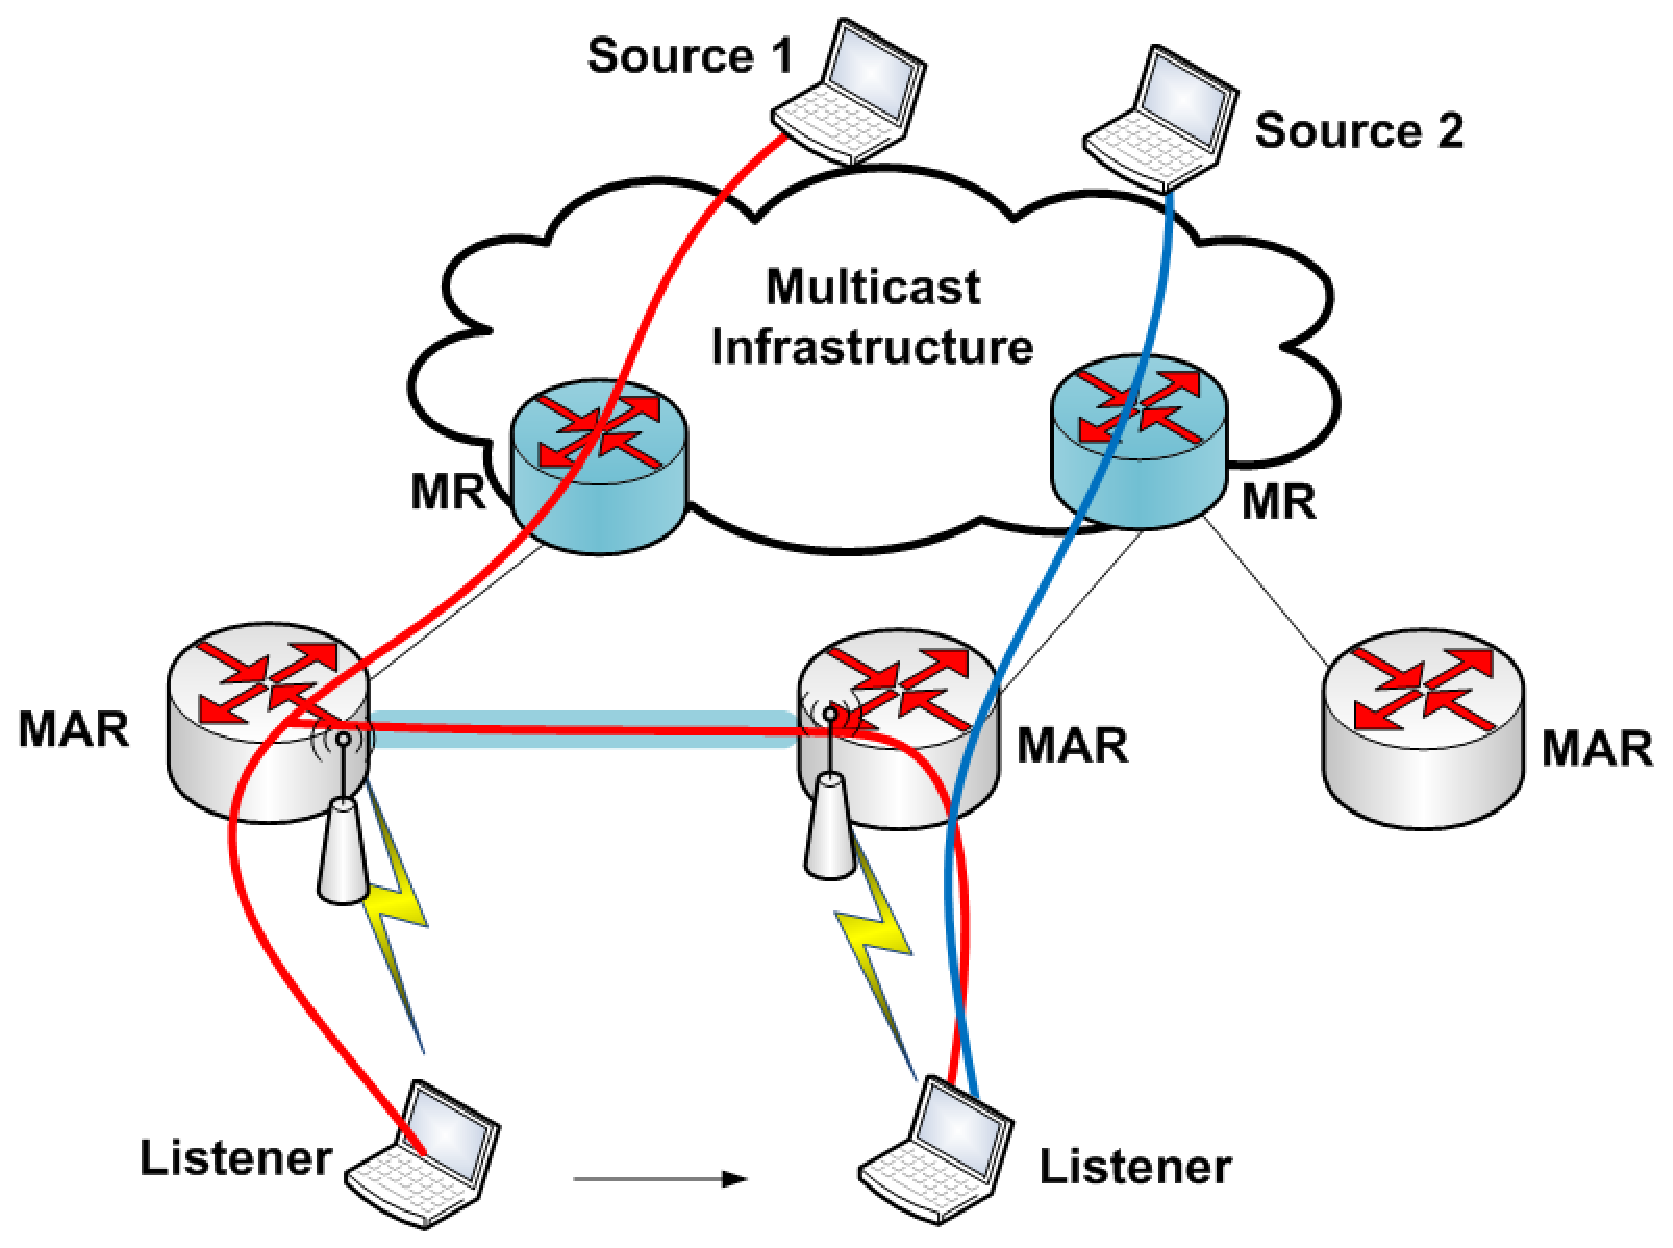
\includegraphics[width=0.50\textwidth]{./Part1/Chapter2/figures/c4_dmm_listener_mld.eps} 
    \caption{Multicast listener mobility in DMM (MLD deployment at MARs).}
     \label{fig:c4_dmm_listener_mld}
  \end{center} 
\end{figure}
However, this mode does not address any multicast-related issues. Among them, we just highlight the following issues: 
\begin{itemize}
\item \textit{Service disruption (and packet loss)}: When a multicast listener moves from the pMAR to the cMAR, several multicast-related procedures need to be executed to allow the listener to continue receiving the ongoing multicast channels. Consequently, it causes a noticeable service disruption (due to the multicast service activation, MLD response delay, and MLD Query/Report transmission). By using the multicast context transfer and the explicit tracking function, the service disruption time could be greatly reduced \cite{Thinh_WCNC_Multicast}. However, in some cases, it is far from the values required by specific services (e.g., interruption-sensitive services). For instance, in \cite{Thinh_ICNS, multicast_DMM_Sergio_PIMRC}, the authors showed that the multicast service disruption time strongly depends on the tunnel delay between the aMAR and cMAR. Hence, by reducing the tunnel delay, the service disruption time can be reduced \cite{Thinh_ICC}.
\item \textit{Non-optimal routing and end-to-end delay}: Since the multicast traffic always traverses the aMAR, it often results in a longer route (e.g., when the source and the listener are close to each other but far from the listener's aMAR). In particular, when considering a significant large domain, it can cause a high end-to-end delay. Therefore, avoiding utilization of the mobility tunnel or shortening the tunnel could help \cite{Thinh_ICC}.  
\item \textit{Tunnel convergence problem}: In case of mobility, the utilization of the mobility tunnel for the multicast flow may result in the tunnel convergence problem. This issue occurs when multiple instances of the same multicast traffic converge to an MAR, leading to the redundant traffic. It is because the multiple MLD proxy instances are installed at the MAR with their upstream interfaces configured to different aMARs. Since the purpose of DMM is moving the mobility anchors from the core to the edge of the networks, the number of mobility anchors in a DMM domain will be much more than that in a PMIPv6 domain. As a consequence, the tunnel convergence problem is supposed to be much more severe than that in PMIPv6, especially in highly mobile regimes. As stated in the DMM requirements \cite{DMM_requirements}, the multicast solutions in DMM should take this issue into consideration. In \cite{Channel_manageable_Seil}, the authors introduced a framework managing all multicast channels and controlling which channel should be received from the multicast infrastructure (for local content) or the previous MAR (for remote content). This solution helps to minimize the multicast traffic duplication. However, as only one upstream interface is configured at a time, it may cause the tunnel convergence problem again when an aggregated MLD Report is sent to the upstream interface. Thus, the tunnel convergence problem cannot be completely avoided. On the other hand, the problem can be solved by using an extension to MLD proxy to support the multiple upstream interfaces \cite{multi_upstream_interface}. In this case, only one proxy instance will be installed at MAR with different upstream interfaces towards different aMARs (and its upstream MR). Hence, the MAR will receive only one instance of the multicast packet. Also, in a DMM environment, it is unfeasible to pre-establish all the tunnels between MARs since the number of MARs is supposed to be large. When considering the MLD proxy supporting multiple upstream interfaces in DMM, it may cause the complex tunnel management (e.g., maintenance of the tunnel and keep alive signaling). Another solution which helps to reduce the number of duplication traffic is proposed in \cite{Thinh_ICNS}.
\end{itemize}

Considering the MR function deployment at MARs, the MAR will decide to get the multicast traffic from an MR for an attached listener based on the Reverse Path Forwarding (RPF) check. As a result, the tunnel convergence, non-optimal route will be avoided. However, the movement of the listener causes the service disruption problem. Additionally, the operators may not want to support the multicast routing function on MAR due to its implementation and operational costs compared to MLD proxy.

\subsubsection{Multicast Source Support in DMM}
Similar to the multicast source mobility in PMIPv6, a limited work has been done for the source mobility in PMIPv6. Also, multicast source mobility in DMM inherits the issues from that in PMIPv6. In \cite{d4.2,multicast_DMM_sergio}, the authors propose to enable the multicast source mobility in a DMM environment by deploying MLD proxy at MAR. In case of handover, the multicast traffic will be routed from the current MAR to the anchor one via the mobility tunnel between them. Although this solution is simple and easy to deploy, it comes up again the sub-optimal routing when the source and listeners, after handover, are attached to the same MAR (but from different anchor MARs). When the MAR acts as an MR, it considers the source as a new source. Thus, it encapsulates the multicast packets and sends them to the RP (in case of ASM). The RP then sends a PIM Join message towards the source's aMAR to establish the SPT. Thus, the traffic first passes the aMAR and then the RP. In addition, if the mobility occurs after the DR's listener switches to the SPT towards source, the mobility will reset the SPT routing state, leading to a significant service disruption and packet loss. In case of SSM, the multicast delivery tree will be reconstructed based on PIM process. Again, it may cause a noticeable service disruption and a high number of lost packets. 
\section{Conclusion}

As more and more applications and services in the Internet are based on the multicast technique, the multicast will play a crucial role in the future networks. So as to provide the multicast service, two groups of protocol need to be deployed: the multicast group membership protocols and the multicast routing protocols. The multicast group membership protocols are used to communicate between the hosts and their routers. Relying on MLDv2, we analyzed the role and operations of these protocols. Using MLDv2 protocol, a host informs its router about its interest of receiving/leaving a multicast group, while an MR manages its membership state information on the attached link. Various multicast routing protocols then have been presented, in which the PIM-SM protocol is insisted. Finally, to avoid deploying a full-stack multicast router in a given network, an MLD proxy is introduced as a lightweight solution. 

Regarding IP mobility management protocols, there are a various IP mobility protocols ranging from the host-based to the network-based, from the centralized to the distributed approach. Typically, PMIPv6 as a network-based mobility management offers advantages compared to the host-based one in terms of complexity of the MN, signaling overhead and handover latency. However, PMIPv6, as a centralized mobility approach, relies on a centralized mobility anchor to support mobility. Thus, it causes several limitations when the number of mobile devices and their traffic demand increase. To tackle these limitations, DMM has been introduced. The research publications showed that DMM is a promising choice for the future networks. 

Based on the analysis regarding IP multicast and IP mobility management protocol, we then highlighted the issues when considering IP multicast in different mobility management protocols. First, we have made a brief introduction on the multicast-related issues as well as the proposals for multicast mobility in MIPv6. We then made an in-depth analysis in PMIPv6 and DMM. In the context of our thesis, we focus on such issues as the multicast service disruption, packet loss, sub-optimal routing, tunnel convergence problem, and leave latency (waste of resources).  
